
\setsecnumdepth{subsection}

\begin{alttitles}

\chapter{Eigenapplications}
\label{ch:eigenapps}

We end this book with a few more ultra-cool real-world applications of linear
algebra. Unlike those in Chapter~\ref{ch:apps}, though, these will all involve
the \textbf{eigenvalue} concepts you learned in Chapter~\ref{ch:eigen}. Our
new ability to penetrate to the heart of a matrix and understand its inner
structure will enable us to do things we could only dream about before.

\pagebreak

\renewcommand{\thesubsection}{V\arabic{subsection}.}%... from subsections
\section{Video compression}

Imagine you owned a business, and you needed to send a $7\times 7$ matrix over
the Internet to one of your customers. Say, this matrix:

\vspace{-.15in}
\begin{align*}
M_1 = 
\begingroup
\renewcommand*{\arraystretch}{1.2}
\begin{bmatrix}
5 & -1 & 45 & 16 & 16 & 3 & 37 \\
3 & -9 & 9  & 27 & -100 & 24 & 601 \\
13 & 0 & 2  & 13 & -18 & 21 & 11 \\
-4 & 33 & 9  & 1 & 4 & 14 & 50 \\
-21 & 51 & 9  & 17 & 5 & 73 & -5 \\
31 & -5 & 9  & -99 & -22 & 1 & 7 \\
6 & 8 & 9  & 24 & 8 & 8 & 8 \\
\end{bmatrix}.
\endgroup
\end{align*}
\vspace{-.15in}

How many numbers in total would you have to send your customer to communicate
the information in this matrix?

Easy question. There are 49 entries in a 7-by-7 matrix, so you need to send 49
numbers. Duh.

\medskip

Now suppose you wanted to send this matrix instead:

\vspace{-.15in}
\begin{align*}
M_2 = 
\begingroup
\renewcommand*{\arraystretch}{1.2}
\begin{bmatrix}
5 & 5 & 10 & -5 & 20 & 500 & 2\frac{1}{2} \\
3 & 3 & 6 & -3 & 12 & 300 & 1\frac{1}{2} \\
13 & 13 & 26 & -13 & 52 & 1300 & 6\frac{1}{2} \\
-4 & -4 & -8 & 4 & -16 & -400 & -2 \\
-21 & -21 & -42 & 21 & -84 & -2100 & -10\frac{1}{2} \\
31 & 31 & 62 & -31 & 124 & 3100 & 15\frac{1}{2} \\
6 & 6 & 12 & -6 & 24 & 600 & 3 \\
\end{bmatrix}.
\endgroup
\end{align*}
\vspace{-.15in}

How many numbers would you have to send this time?

If you answered, ``again, 49,'' take another look. $M_2$ is way different than
$M_1$, because it has a very regular structure. Look at $M_2$'s first
(leftmost) column. Then realize that its second column is identical to the
first. Then further realize that its third column is exactly \textit{twice} the
first. And its fourth column is \textit{negative} the first. And its last three
columns are four times, a hundred times, and one-half times the first column,
respectively.

So if your customer knew the matrix would have this type of structure, I claim
you could send them all the necessary information in just \textit{fourteen}
numbers instead of 42. Here's how:

\begin{compactenum}
\item First, send them the first column: $[\ 5\ \ 3\ \ 13\ \ -4\ \ -21\ \ 31\ \
6\ ]$. That's seven numbers.
\index{Oakenshield, Thorin}
\item Then, send them the multiplier for each of the other columns. Namely, $[\
1\ \ 1\ \ 2\ \ -1\ \ 4\ \ 100\ \ \frac{1}{2}\ ]$. That, too, is seven
numbers.\footnote{Yeah, yeah, I know we could omit the first ``1'' in this
second set of seven, because the customer will know that the first column
should be multiplied by 1 without us having to tell them. That's a detail, and
it's actually messier to take advantage of that. Thirteen is unlucky anyway --
ask Thorin Oakenshield if you don't believe me.}

\end{compactenum}

\index{outer product}

From these fourteen numbers alone, the customer can reconstruct the original
matrix. All they have to do is compute the outer product (recall
p.~\pageref{outerProduct}) of the two 7-element vectors they received:

\vspace{-.15in}
\begin{gather*}
\begin{bmatrix}
5 \\ 3 \\ 13 \\ -4 \\ -21 \\ 31 \\ 6 \\
\end{bmatrix} \ \textrm{\textbullet} \ 
\begin{bmatrix}
1 & 1 & 2 & -1 & 4 & 100 & \frac{1}{2} \\
\end{bmatrix} =\\
\begingroup
\renewcommand*{\arraystretch}{1.2}
\begin{bmatrix}
5 & 5 & 10 & -5 & 20 & 500 & 2\frac{1}{2} \\
3 & 3 & 6 & -3 & 12 & 300 & 1\frac{1}{2} \\
13 & 13 & 26 & -13 & 52 & 1300 & 6\frac{1}{2} \\
-4 & -4 & -8 & 4 & -16 & -400 & -2 \\
-21 & -21 & -42 & 21 & -84 & -2100 & -10\frac{1}{2} \\
31 & 31 & 62 & -31 & 124 & 3100 & 15\frac{1}{2} \\
6 & 6 & 12 & -6 & 24 & 600 & 3 \\
\end{bmatrix}.
\endgroup
\end{gather*}
\vspace{-.15in}

\medskip
\label{rank-deficient}

What's going on here? Simply put, $M_2$ has \textit{less information} in it
than $M_1$ does, despite the fact that they are ostensibly the same size. In
fact, you may have realized that $M_2$ is a \textbf{rank-1} matrix. It has only
one linearly independent column: all the others are simply (scaled) copies of
it. This is what a rank-deficient matrix fundamentally is: a matrix that can
have some of its entries ``squeezed'' out of it without losing any information.

\smallskip

$M_1$ and $M_2$ represent the far extremes of this phenomenon. $M_1$ is full
rank (rank-7), and $M_2$ is just rank-1. In general, a $7\times 7$
rank-deficient matrix might not be \textit{as} deficient as $M_2$ is: it could
have a rank anywhere from 1 to 6.

\smallskip

Incidentally, 14 numbers might not seem like that big a savings over 49 (it's
only 3.5 times fewer entries), but consider what happens as the matrix gets
larger. Suppose it were $1920\times 1920$. Transmitting a rank-1 matrix of that
size would require $1920+1920=$\ 3,840 numbers to go across the wire. But a
full-rank matrix of that size would need \textit{3,686,400} entries. That's
nearly 1,000 times as much data.

\subsection{Enter Netflix}

\index{frame (of a video)}
\index{gray scale}
\index{bit / byte}

Now what's the application here? Well, it's probably one you use every day.
Suppose your aforementioned business is a video streaming service, and your
customer is watching one of your videos. The matrix we've been talking about is
one \textbf{frame} of this video. For simplicity, we'll consider images
(frames) that are in \textbf{gray scale} rather than color. Each \textbf{pixel}
of the image is represented by a single number on some scale: perhaps 0
indicates a pitch black pixel in the current frame, and 255 is bright white,
and all the numbers in between are shades of gray.\footnote{Why a range of 0
through 255? Because as you may remember from Chapters 6 and 7 of \textit{A
Cool Brisk Walk}, that's how many different values can fit in a single byte (8
bits) of data.}

If each frame of our movie is a $1920\times 1920$-pixel square\footnote{At this
point it may occur to you that when you watch a movie, your screen typically
isn't perfectly square, but rectangular. Its \index{aspect ratio}
\textbf{aspect ratio} (width-to-height) might be, say, 1.875:1, which yields a
$1920\times 1024$ canvas. \\ \indent When your matrix isn't square, instead of using
the eigenvalue decomposition, as we learned last chapter, we can use the
\index{singular value decomposition (SVD)} \textbf{singular value decomposition
(SVD)}, a very closely related technique. In fact, the ``singular values'' and
``singular vectors'' that the SVD gives you are exactly the same thing as
eigenvalues and eigenvectors for a non-square matrix.}, and we're shoveling 30
frames per second at our viewer, that would be about 105 Megabytes of
information \textit{every second} we'd be trying to send. The Internet
ain't got no time for that.

So we'd like to instead send a compressed version of each frame: a matrix whose
rank is far less than 1,920 and yet which looks pretty close to the original.
Our problem thus reduces to: \textit{what matrix, of the same size as the
original image's matrix but of at most rank-k (for some number k) is the
``closest'' to the original?}

\subsection{Yet another norm}

\index{Frobenius norm}
\index{norm (of a matrix)}
\index{Euclidean norm}

First, we have to settle on what we mean by one matrix being ``close'' to
another. Here, we'll subtract one matrix from the other, and then take the
\textbf{Frobenius norm} of this difference. Subtracting matrices, of course, is
just the inverse of adding them (p.~\pageref{matrixAddition}): we do it element
by element and get a matrix of the differences. The ``Frobenius norm'' (which
always sounded to me like a character from a Willy Wonka story, btw) is just
what you would expect it to be: the square-root of the sum of all these squared
differences. In fact it's exactly like the Euclidean norm of a vector
(p.~\pageref{Euclideannorm}), except that we have a two-dimensional pane of
entries to work with instead of just a one-dimensional list.

To be concrete, let's say we have a matrix $M$, and an ``approximation'' to
matrix $M$ called $\hat{M}$, with the following values:

\vspace{-.15in}
\begin{align*}
M =
\begin{bmatrix}
17 & 2 \\
-3 & 6 \\
\end{bmatrix}, \quad
\hat{M} =
\begin{bmatrix}
14 & 4 \\
-5 & -1 \\
\end{bmatrix}, 
\end{align*}
\vspace{-.15in}

How ``close'' are these two matrices to each other? To quantify this, we first
subtract one from the other (doesn't matter which order):

\vspace{-.15in}
\begin{align*}
M - \hat{M} =
\begin{bmatrix}
3 & -2 \\
2 & 7 \\
\end{bmatrix}.
\end{align*}
\vspace{-.15in}

And then we take the square-root of the sum of the squared entries to give us
the Frobenius norm:

\vspace{-.15in}
\begin{align*}
{\left\lVert{M - \hat{M}}\right\rVert_F} =
\sqrt{3^2 + -2^2 + 2^2 + 7^2} = 8.124.
\end{align*}
\vspace{-.15in}

This measure passes a quick sanity check: the further apart the entries of $M$
and $\hat{M}$ at a particular row and column, the larger the difference that is
added towards the Frobenius norm. So this metric gives pairs of matrices whose
entries are more similar to each other a lower overall norm, indicating a
higher similarity.

\subsection{Best low-rank matrix approximations}

\index{dominant eigenvector}

And now for our eigenstuff. Recall (p.~\pageref{theScoopAboutEigenvectors} and
following) that every eigenvector of a matrix has a corresponding eigenvalue,
and that we could arrange these eigenvectors by decreasing eigenvalue if we
like. The one with the largest eigenvalue had the special name ``dominant
eigenvector.'' I'll also refer to ``the top eigenvector,'' ``the top two
eigenvectors,'' ``the top ten eigenvectors,'' and so forth, by which I just
mean ``the $k$ eigenvectors with the highest eigenvalues.''

Okay. It turns out that the best rank-1 approximation to a square matrix (where
``best'' means ``closest to the original when using the Frobenius norm'') is
\textit{the dominant eigenvector, times its eigenvalue, times the transpose of
the dominant eigenvector.} To illustrate, let's say we had this $5\times 5$
matrix\footnote{You may notice that this example matrix happens to be
\textit{symmetric}. Things actually get slightly weird for non-symmetric
matrices, in which case you can again turn to the SVD,\index{singular value
decomposition (SVD)} which is almost the same thing as the
\index{eigendecomposition (of a matrix)} eigendecomposition.}:

\vspace{-.15in}
\label{Amatrix}
\begin{align*}
A =
\begin{bmatrix}
12 & 2 & 1 & 9 & 13 \\
2 & 20 & 12 & 7 & 5 \\
1 & 12 & 6 & -4 & 5 \\
9 & 7 & -4 & 8 & 8 \\
13 & 5 & 5 & 8 & 13 \\
\end{bmatrix}
,
\end{align*}
\vspace{-.15in}

and we wanted the best rank-1 approximation to it. We ask Python for its
dominant eigenvector, and the corresponding eigenvalue, and get this:

\vspace{-.15in}
\begin{align*}
\overrightarrow{x_1} = 
\begin{bmatrix}
.462 \\ .538 \\ .257 \\ .38 \\ .535 \\
\end{bmatrix}, \quad
\lambda_1 = 37.363.
\end{align*}
\vspace{-.15in}

Multiplying these out as indicated above, we get:

\vspace{-.15in}
\begin{gather*}
\overrightarrow{x_1} \ \textrm{\textbullet} \  \begin{bmatrix} \lambda_1
\end{bmatrix} \ \textrm{\textbullet} \  \overrightarrow{x_1}^\intercal =\\
\begin{bmatrix}
.462 \\ .538 \\ .257 \\ .38 \\ .535 \\
\end{bmatrix} \ \textrm{\textbullet}\ 
\begin{bmatrix}
37.363
\end{bmatrix} \ \textrm{\textbullet}\ 
\begin{bmatrix}
.462 & .538 & .257 & .38 & .535 \\
\end{bmatrix} = \\
\begin{bmatrix}
7.963 & 9.288 & 4.441 & 6.563 & 9.222\\
9.288 & 10.834 & 5.18 & 7.655 & 10.757\\
4.441 & 5.18 & 2.477 & 3.66 & 5.143\\
6.563 & 7.655 & 3.66 & 5.409 & 7.6 \\
9.222 & 10.757 & 5.143 & 7.6 & 10.68 \\
\end{bmatrix}.
\end{gather*}
\vspace{-.05in}

\index{Spectral Theorem}

Take careful note to see that \textit{this is actually the \textbf{Spectral
Theorem} in action} (from p.~\pageref{SpectralTheorem}) but using only a subset
of the eigenvectors/eigenvalues (namely, the top one) instead of all of them.
(This is why I put the top eigenvalue, 37.363, into a $1\times 1$ matrix in the
equation above -- to help you see that connection.)

\medskip

Now how close is this approximation to our original $A$ matrix? Not that great,
actually. If you run your eyes over the entries, and compare to $A$
(p.~\pageref{Amatrix}) it doesn't even look like it's trying very hard. The
Frobenius norm of the difference between the two, by the way, is a whopping
573.04, which tells you that limiting ourselves to rank-1 isn't producing a
very good approximation. We wouldn't want to send such an image to our viewer,
even though it would only take 10 bytes instead of 25, because they might not
even know whether they were on HBO or the Disney Channel.

\bigskip

Okay, let's move up to rank-2 then. What's the closest rank-2 matrix to our
original? Python says the second highest eigenvalue (and its eigenvector) are:

\vspace{-.15in}
\begin{align*}
\overrightarrow{x_2} = 
\begin{bmatrix}
-.458 \\ .658 \\ .448 \\ -.266 \\ -.293 \\
\end{bmatrix}, \quad
\lambda_2 = 27.712.
\end{align*}
\vspace{-.15in}

Adding this second eigenvector into the mix, we get:

\vspace{-.15in}
\begin{gather*}
\begin{bmatrix}
| & | \\[6pt]
\overrightarrow{\textbf{x}_{1}} &
\overrightarrow{\textbf{x}_{2}} \\
| & | \\[6pt]
\end{bmatrix} \ \textrm{\textbullet}\ 
\begin{bmatrix}
\lambda_1 & 0 \\
0 & \lambda_2 \\
\end{bmatrix} \ \textrm{\textbullet}\ 
\begin{bmatrix}
| & | \\[6pt]
\overrightarrow{\textbf{x}_{1}} &
\overrightarrow{\textbf{x}_{2}} \\
| & | \\[6pt]
\end{bmatrix}^\intercal = \\
\small
\begingroup
\setlength\arraycolsep{2pt}
\begin{bmatrix}
.462 & -.458 \\
.538 & .658 \\
.257 & .448 \\
.38 & -.266 \\
.535 & -.293 \\
\end{bmatrix} \ \textrm{\textbullet}\ 
\begin{bmatrix}
37.363 & 0 \\
0 & 27.712 \\
\end{bmatrix} \ \textrm{\textbullet}\ 
\begin{bmatrix}
.462 & .538 & .257 & .38 & .535 \\
-.458 & .658 & .448 & -.266 & -.293 \\
\end{bmatrix}\endgroup\\
=
\begin{bmatrix}
 12.515 & 2.748 & -0.011 & 9.211 & 12.138 \\
 2.748 & 20.231 & 11.577 & 3.849 & 6.567 \\
 -0.011 & 11.577 & 6.831 & 1.07 & 2.291 \\
 9.211 & 3.849 & 1.07 & 6.95 & 9.297 \\
 12.138 & 6.567 & 2.291 & 9.297 & 12.548 \\
\end{bmatrix}.
\end{gather*}
\vspace{-.05in}

Now we're talking. Flip back and forth between those numbers and the original
$A$ on p.~\pageref{Amatrix}, and you'll see that with just two eigenvectors,
we're starting to get a remarkably close approximation. Frobenius just
plummeted to 101.62. Repeating this for the best rank-3 approximation, we get:

\vspace{-.15in}
\begin{gather*}
\begin{bmatrix}
| & | & | \\[6pt]
\overrightarrow{\textbf{x}_{1}} &
\overrightarrow{\textbf{x}_{2}} &
\overrightarrow{\textbf{x}_{3}} \\
| & | & | \\[6pt]
\end{bmatrix} \ \textrm{\textbullet}\ 
\begin{bmatrix}
\lambda_1 & 0 & 0 \\
0 & \lambda_2 & 0 \\
0 & 0 & \lambda_3 \\
\end{bmatrix} \ \textrm{\textbullet}\ 
\begin{bmatrix}
| & | & | \\[6pt]
\overrightarrow{\textbf{x}_{1}} &
\overrightarrow{\textbf{x}_{2}} &
\overrightarrow{\textbf{x}_{3}} \\
| & | & | \\[6pt]
\end{bmatrix}^\intercal = \\
\begingroup
\setlength\arraycolsep{2pt}
\footnotesize
\begin{bmatrix}
.462 & -.458 & .156 \\
.538 & .658 & -.33 \\
.257 & .448 & .525 \\
.38 & -.266 & -.651 \\
.535 & -.293 & .408 \\
\end{bmatrix} \ \textrm{\textbullet}\ 
\begin{bmatrix}
37.363 & 0 & 0 \\
0 & 27.712 & 0 \\
0 & 0 & 7.6 \\
\end{bmatrix} \ \textrm{\textbullet}\ 
\begin{bmatrix}
.462 & .538 & .257 & .38 & .535 \\
-.458 & .658 & .448 & -.266 & -.293 \\
.156 & -.33 & .525 & -.651 & .408 \\
\end{bmatrix} \endgroup \\
=
\begin{bmatrix}
12.701 & 2.356 & 0.612 & 8.438 & 12.623 \\
 2.356 & 21.06 & 10.259 & 5.484 & 5.542 \\
 0.612 & 10.259 & 8.925 & -1.528 & 3.921 \\
 8.438 & 5.484 & -1.528 & 10.173 & 7.276 \\
 12.623 & 5.542 & 3.921 & 7.276 & 13.815 \\
\end{bmatrix},
\end{gather*}
\vspace{-.15in}

which is even closer, with a Frobenius norm of just 59.07.

\bigskip

Each time we add another eigenvector, we give our approximation another degree
of freedom which it can use to bend closer to the original. And finally, if we
use all 5, we of course get the original matrix back:

\vspace{-.15in}
\footnotesize
\begin{gather*}
\begin{bmatrix}
| & | & | & | & | \\[6pt]
\overrightarrow{\textbf{x}_{1}} &
\overrightarrow{\textbf{x}_{2}} &
\overrightarrow{\textbf{x}_{3}} &
\overrightarrow{\textbf{x}_{4}} &
\overrightarrow{\textbf{x}_{3}} \\
| & | & | & | & | \\[6pt]
\end{bmatrix} \ \textrm{\textbullet}\ 
\begin{bmatrix}
\lambda_1 & 0 & 0 & 0 & 0 \\
0 & \lambda_2 & 0 & 0 & 0 \\
0 & 0 & \lambda_3 & 0 & 0 \\
0 & 0 & 0 & \lambda_4 & 0 \\
0 & 0 & 0 & 0 & \lambda_5 \\
\end{bmatrix} \ \textrm{\textbullet}\ 
\begin{bmatrix}
| & | & | & | & | \\[6pt]
\overrightarrow{\textbf{x}_{1}} &
\overrightarrow{\textbf{x}_{2}} &
\overrightarrow{\textbf{x}_{3}} &
\overrightarrow{\textbf{x}_{4}} &
\overrightarrow{\textbf{x}_{5}} \\
| & | & | & | & | \\[6pt]
\end{bmatrix}^\intercal = \\
\begingroup
\setlength\arraycolsep{2pt}
\footnotesize
\begin{bmatrix}
-0.462 & -0.458 & 0.156 & 0.735 & -0.109 \\
 -0.538 & 0.658 & -0.33 & 0.082 & -0.402 \\
 -0.257 & 0.448 & 0.525 & 0.105 & 0.668 \\
 -0.38 & -0.266 & -0.651 & -0.181 & 0.572 \\
 -0.535 & -0.293 & 0.408 & -0.639 & -0.23 &  \\
\end{bmatrix}\endgroup \ \textrm{\textbullet} \quad \quad \quad \quad \quad \quad \quad \quad
\quad \quad
\\
\quad \quad \quad \quad \quad \quad \quad \quad
\quad \quad
\begingroup
\setlength\arraycolsep{2pt}
\begin{bmatrix}
37.363 & 0 & 0 & 0 & 0 \\
0 & 27.712 & 0 & 0 & 0 \\
0 & 0 & 7.599 & 0 & 0 \\
0 & 0 & 0 & -.151 & 0 \\
0 & 0 & 0 & 0 &  -6.523 \\
\end{bmatrix}\endgroup \ \textrm{\textbullet} \quad \quad \quad \quad \quad \quad \quad \quad
\quad \quad
\\
\end{gather*}
\pagebreak
\begin{gather*}
\quad \quad \quad \quad \quad \quad \quad \quad \quad \quad \quad \quad
\begingroup
\setlength\arraycolsep{2pt}
\begin{bmatrix}
-0.462 & -0.538 & -0.257 & -0.38 & -0.535 \\
 -0.458 & 0.658 & 0.448 & -0.266 & -0.293 \\
 0.156 & -0.33 & 0.525 & -0.651 & 0.408 \\
 0.735 & 0.082 & 0.105 & -0.181 & -0.639 \\
 -0.109 & -0.402 & 0.668 & 0.572 & -0.23 \\
\end{bmatrix}\endgroup = \\
\normalsize
\begin{bmatrix}
12 & 2 & 1 & 9 & 13 \\
2 & 20 & 12 & 7 & 5 \\
1 & 12 & 6 & -4 & 5 \\
9 & 7 & -4 & 8 & 8 \\
13 & 5 & 5 & 8 & 13 \\
\end{bmatrix} = A \quad \checkmark
\end{gather*}
\vspace{-.05in}

\normalsize
by the Spectral Theorem. (And a Frobenius norm of 0.)

\bigskip
\bigskip

Finally, let's look at this work on an actual image.
Figure~\ref{fig:stormtrooper} shows a $1800\times 1800$ gray scale still
frame from a movie. At 1 byte (8 bits) per pixel, the entire original image
would take 3.24 MBytes to transmit in full. That's a lot of data for one frame
of a movie that the viewer will only see for $\frac{1}{30}^\textrm{th}$ of a
second.

\begin{figure}[hb]
\centering

\includegraphics[width=0.5\textwidth]{stormtrooper.png}
\caption{A 3,240,000-byte gray scale image.}
\label{fig:stormtrooper}
\end{figure}

Let's see if we can do better. Figure~\ref{fig:approximations} starts with a
lowly rank-1 matrix (using just the dominant eigenvector), and then increases
the rank as the images move left-to-right down the page.

\begin{figure}[H]
\centering
\begin{tabular}{ccc}
\scriptsize{Rank-1 (3600 bytes)} &
\scriptsize{Rank-2 (7200 bytes)} &
\scriptsize{Rank-3 (10,800 bytes)} \\

\includegraphics[width=0.3\textwidth]{approx01.png} &

\includegraphics[width=0.3\textwidth]{approx02.png} &

\includegraphics[width=0.3\textwidth]{approx03.png}\\
\smallskip
\scriptsize{Rank-6 (21,600 bytes)} &
\scriptsize{Rank-9 (32,400 bytes)} &
\scriptsize{Rank-12 (43,200 bytes)} \\
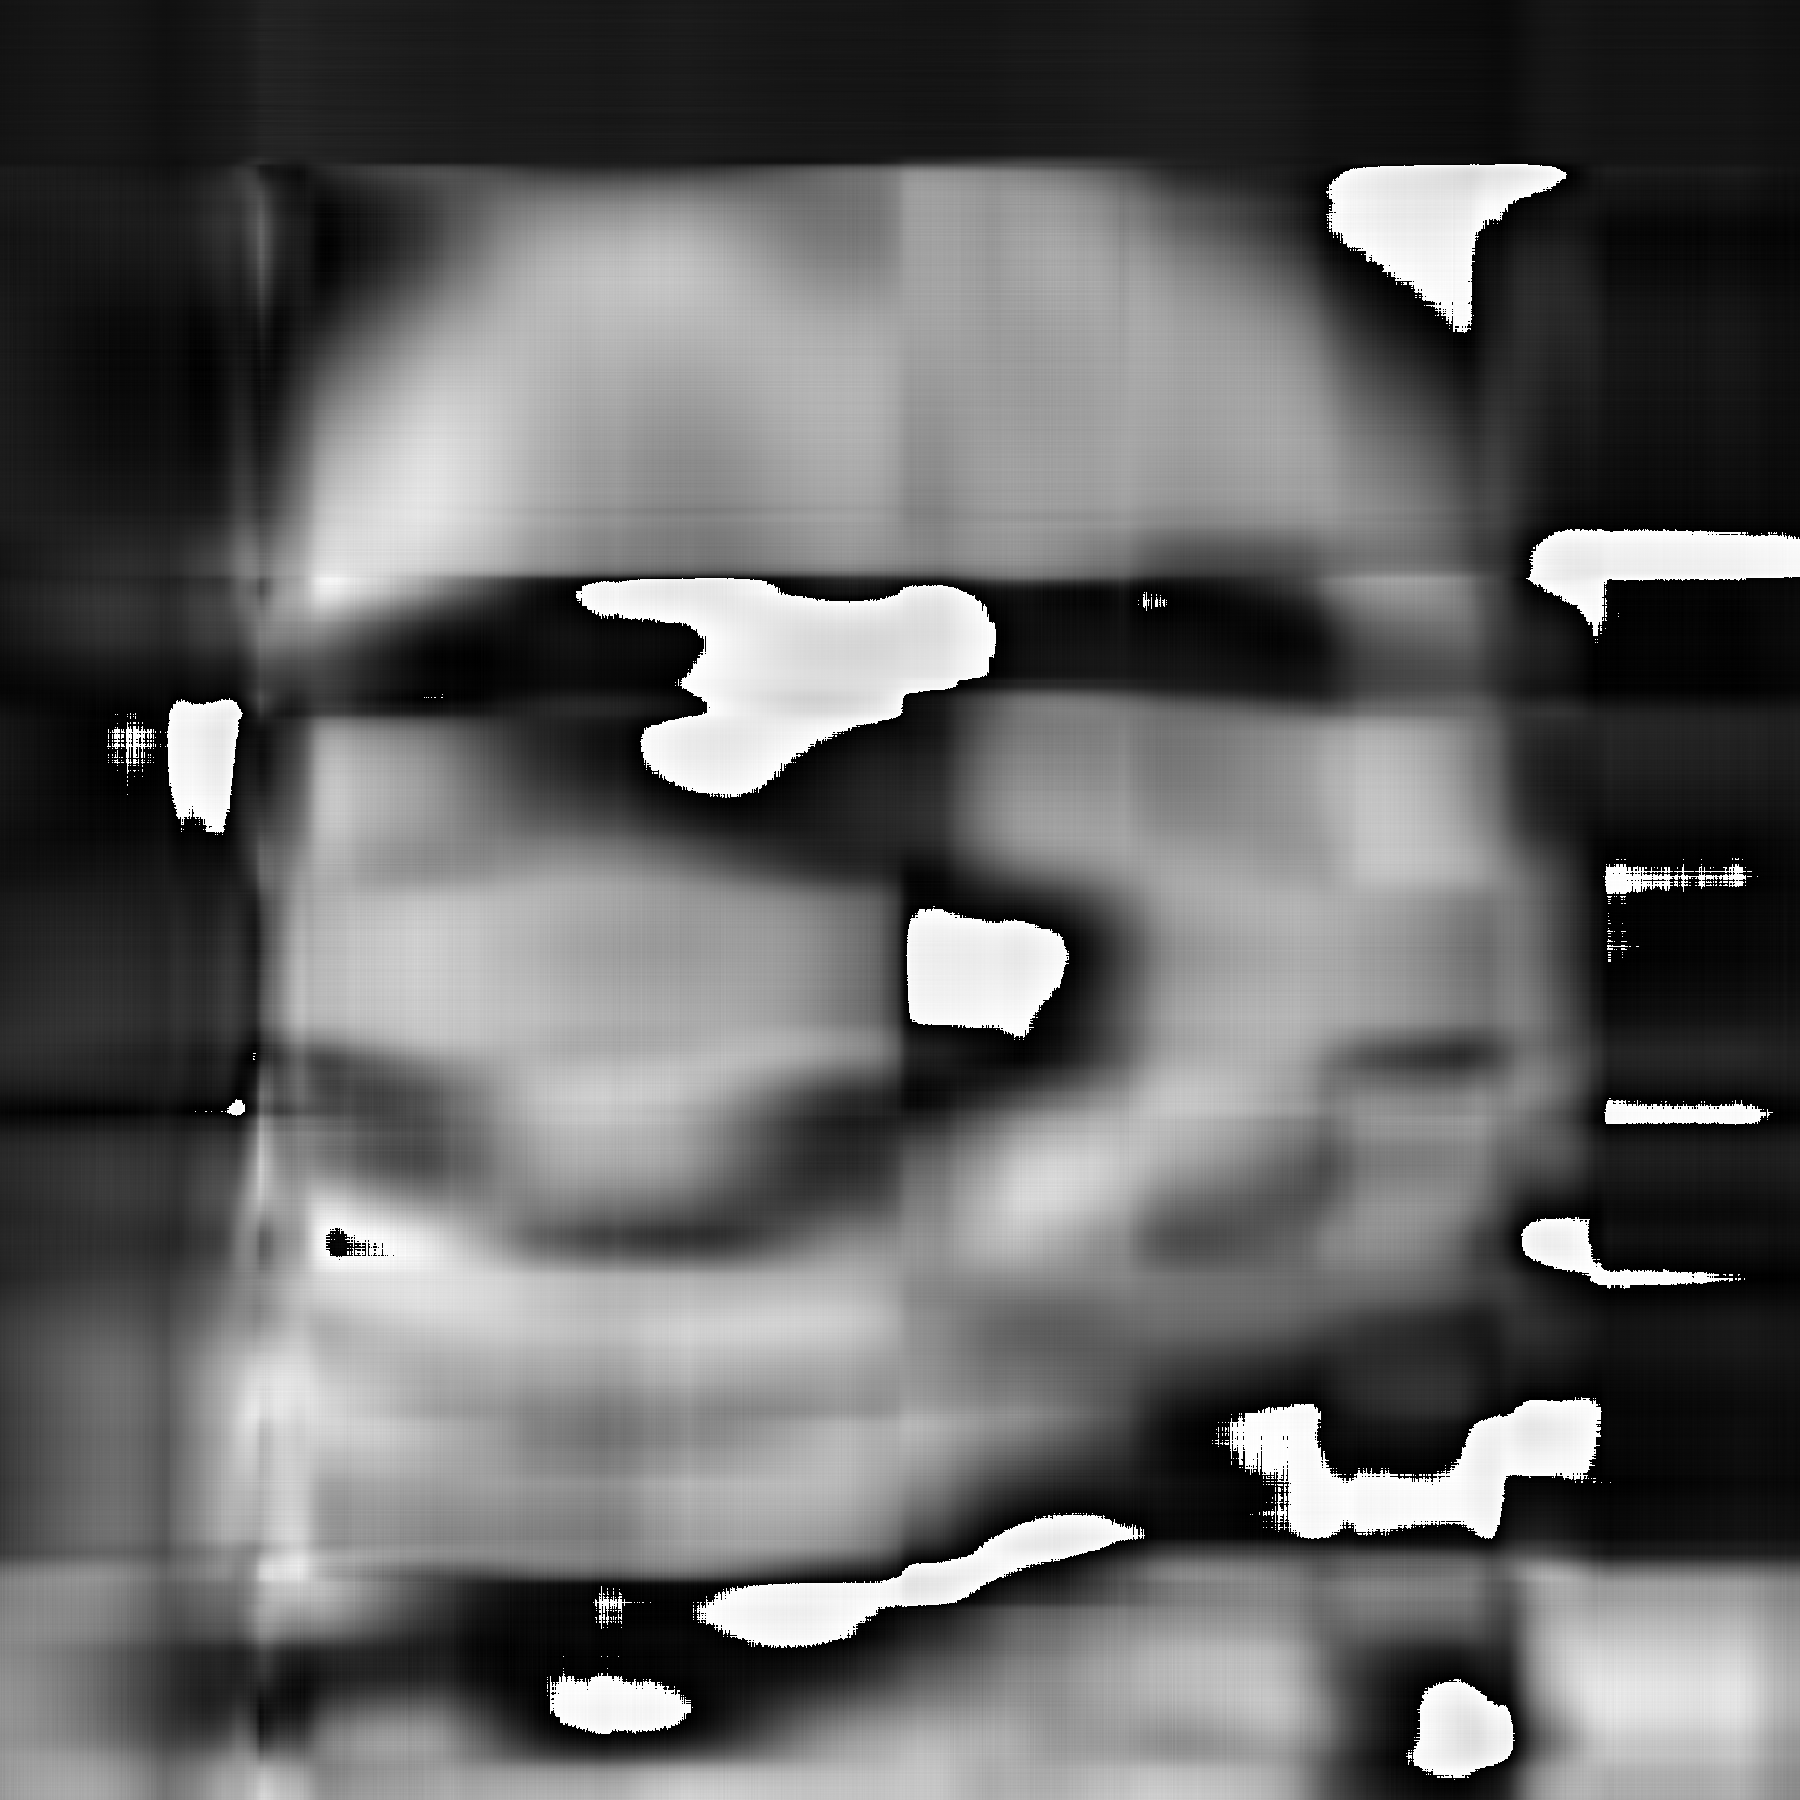
\includegraphics[width=0.3\textwidth]{approx06.png} &
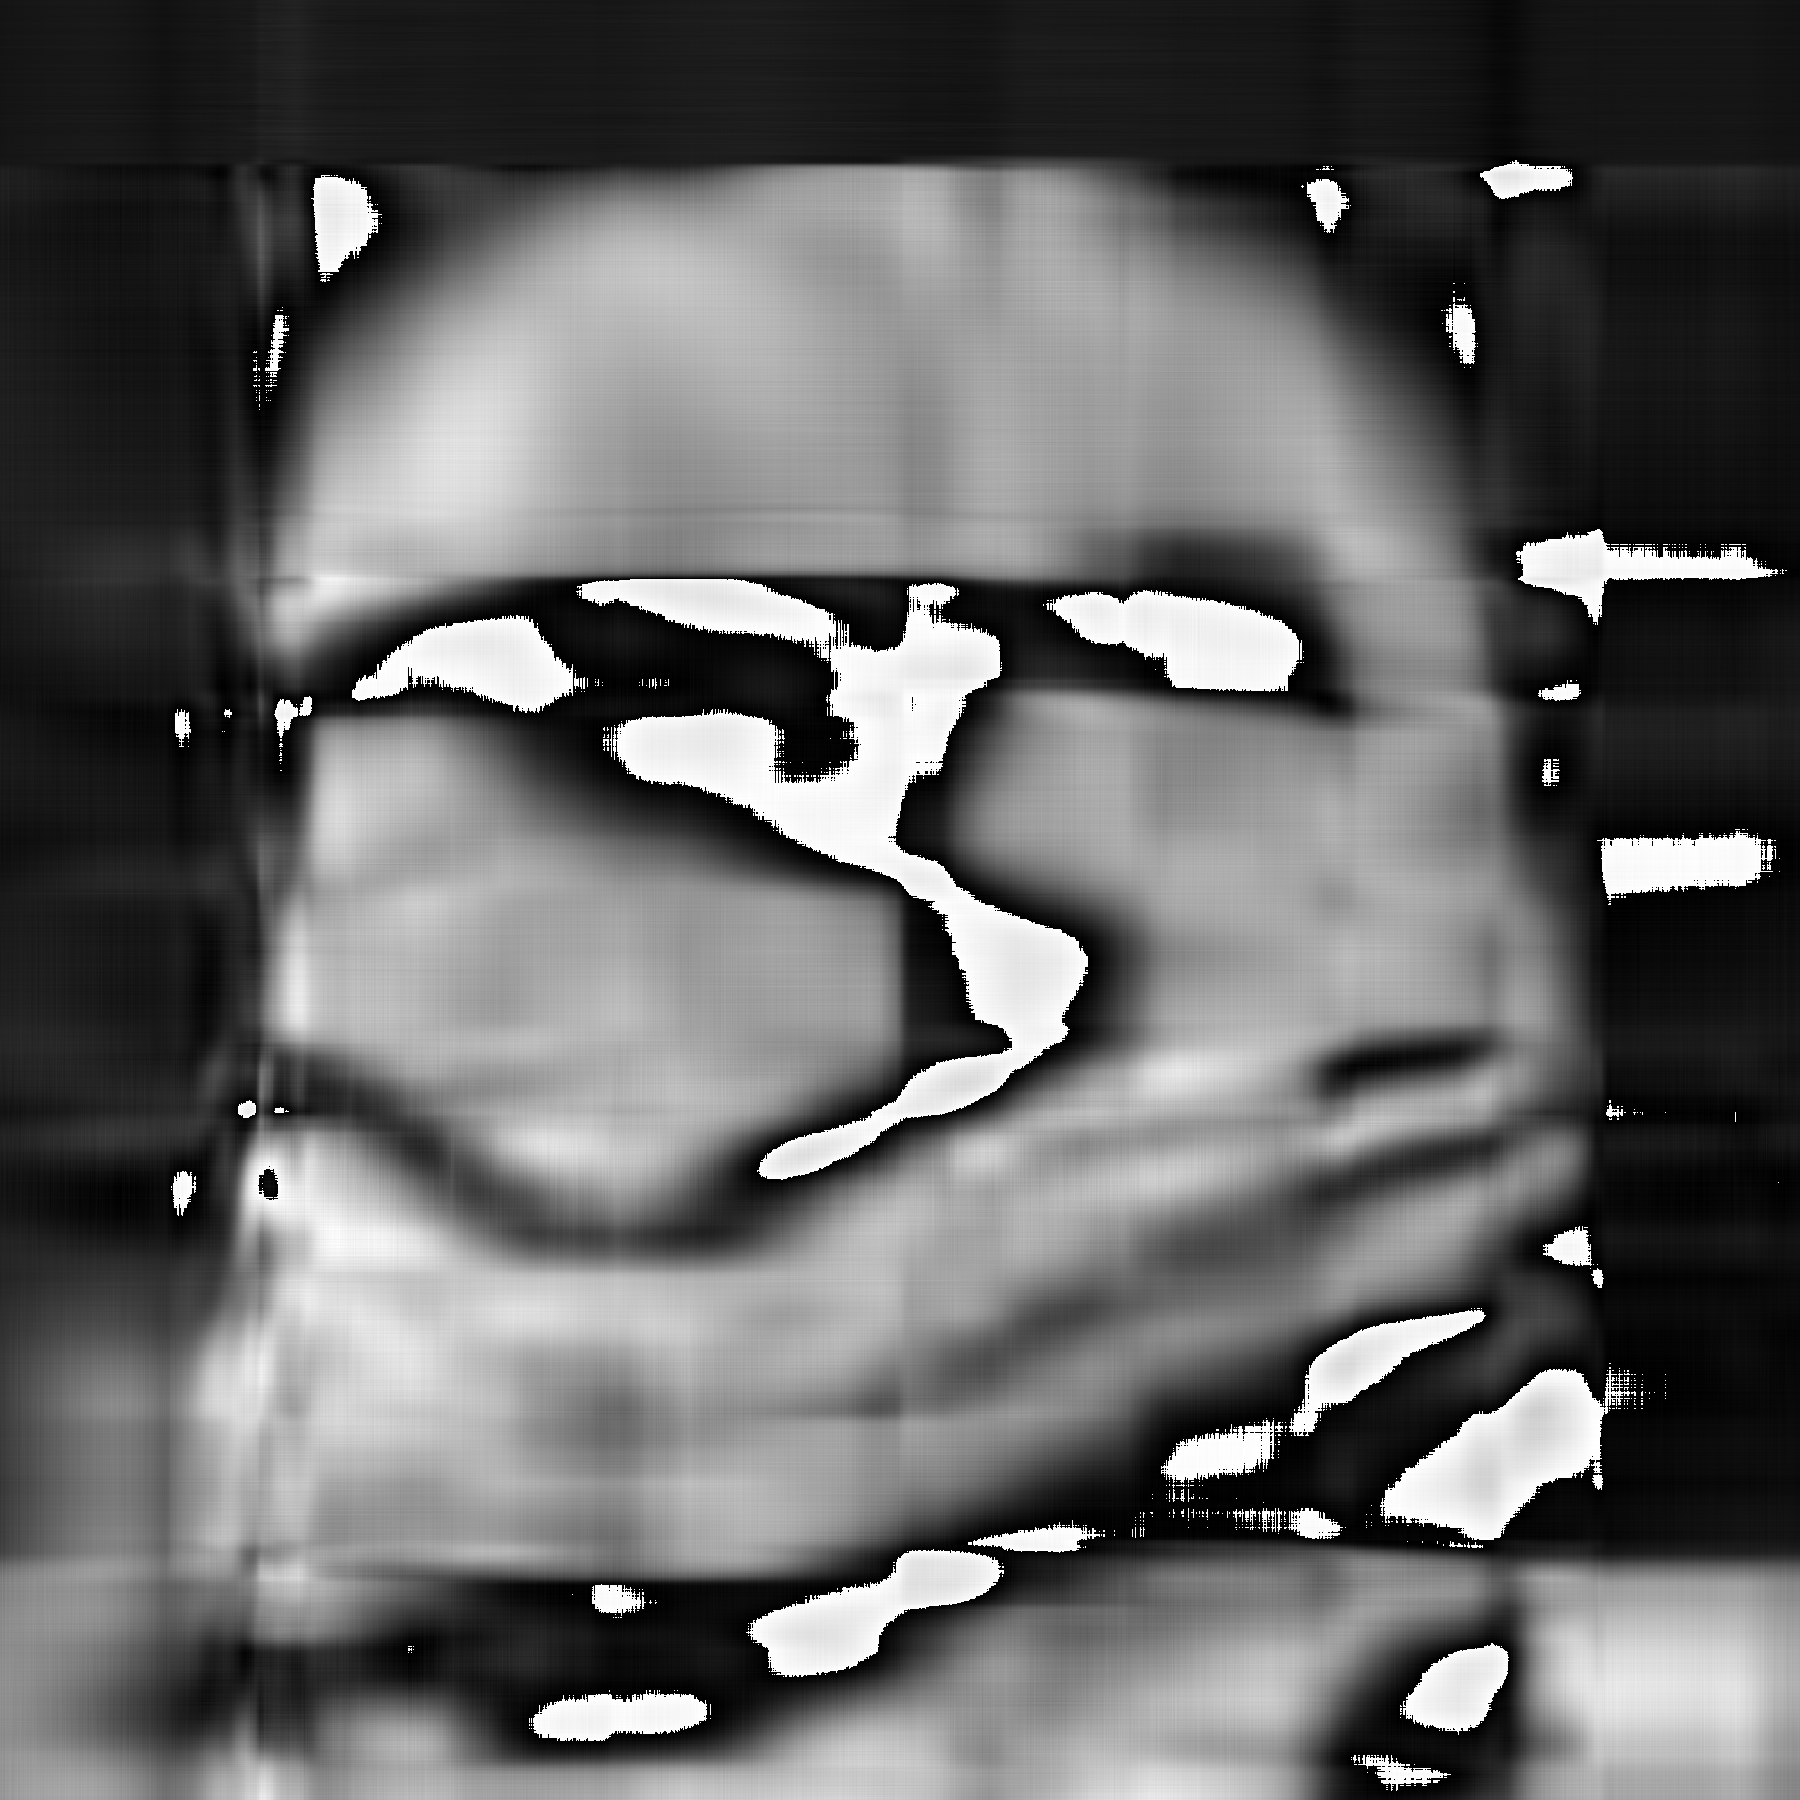
\includegraphics[width=0.3\textwidth]{approx09.png} &
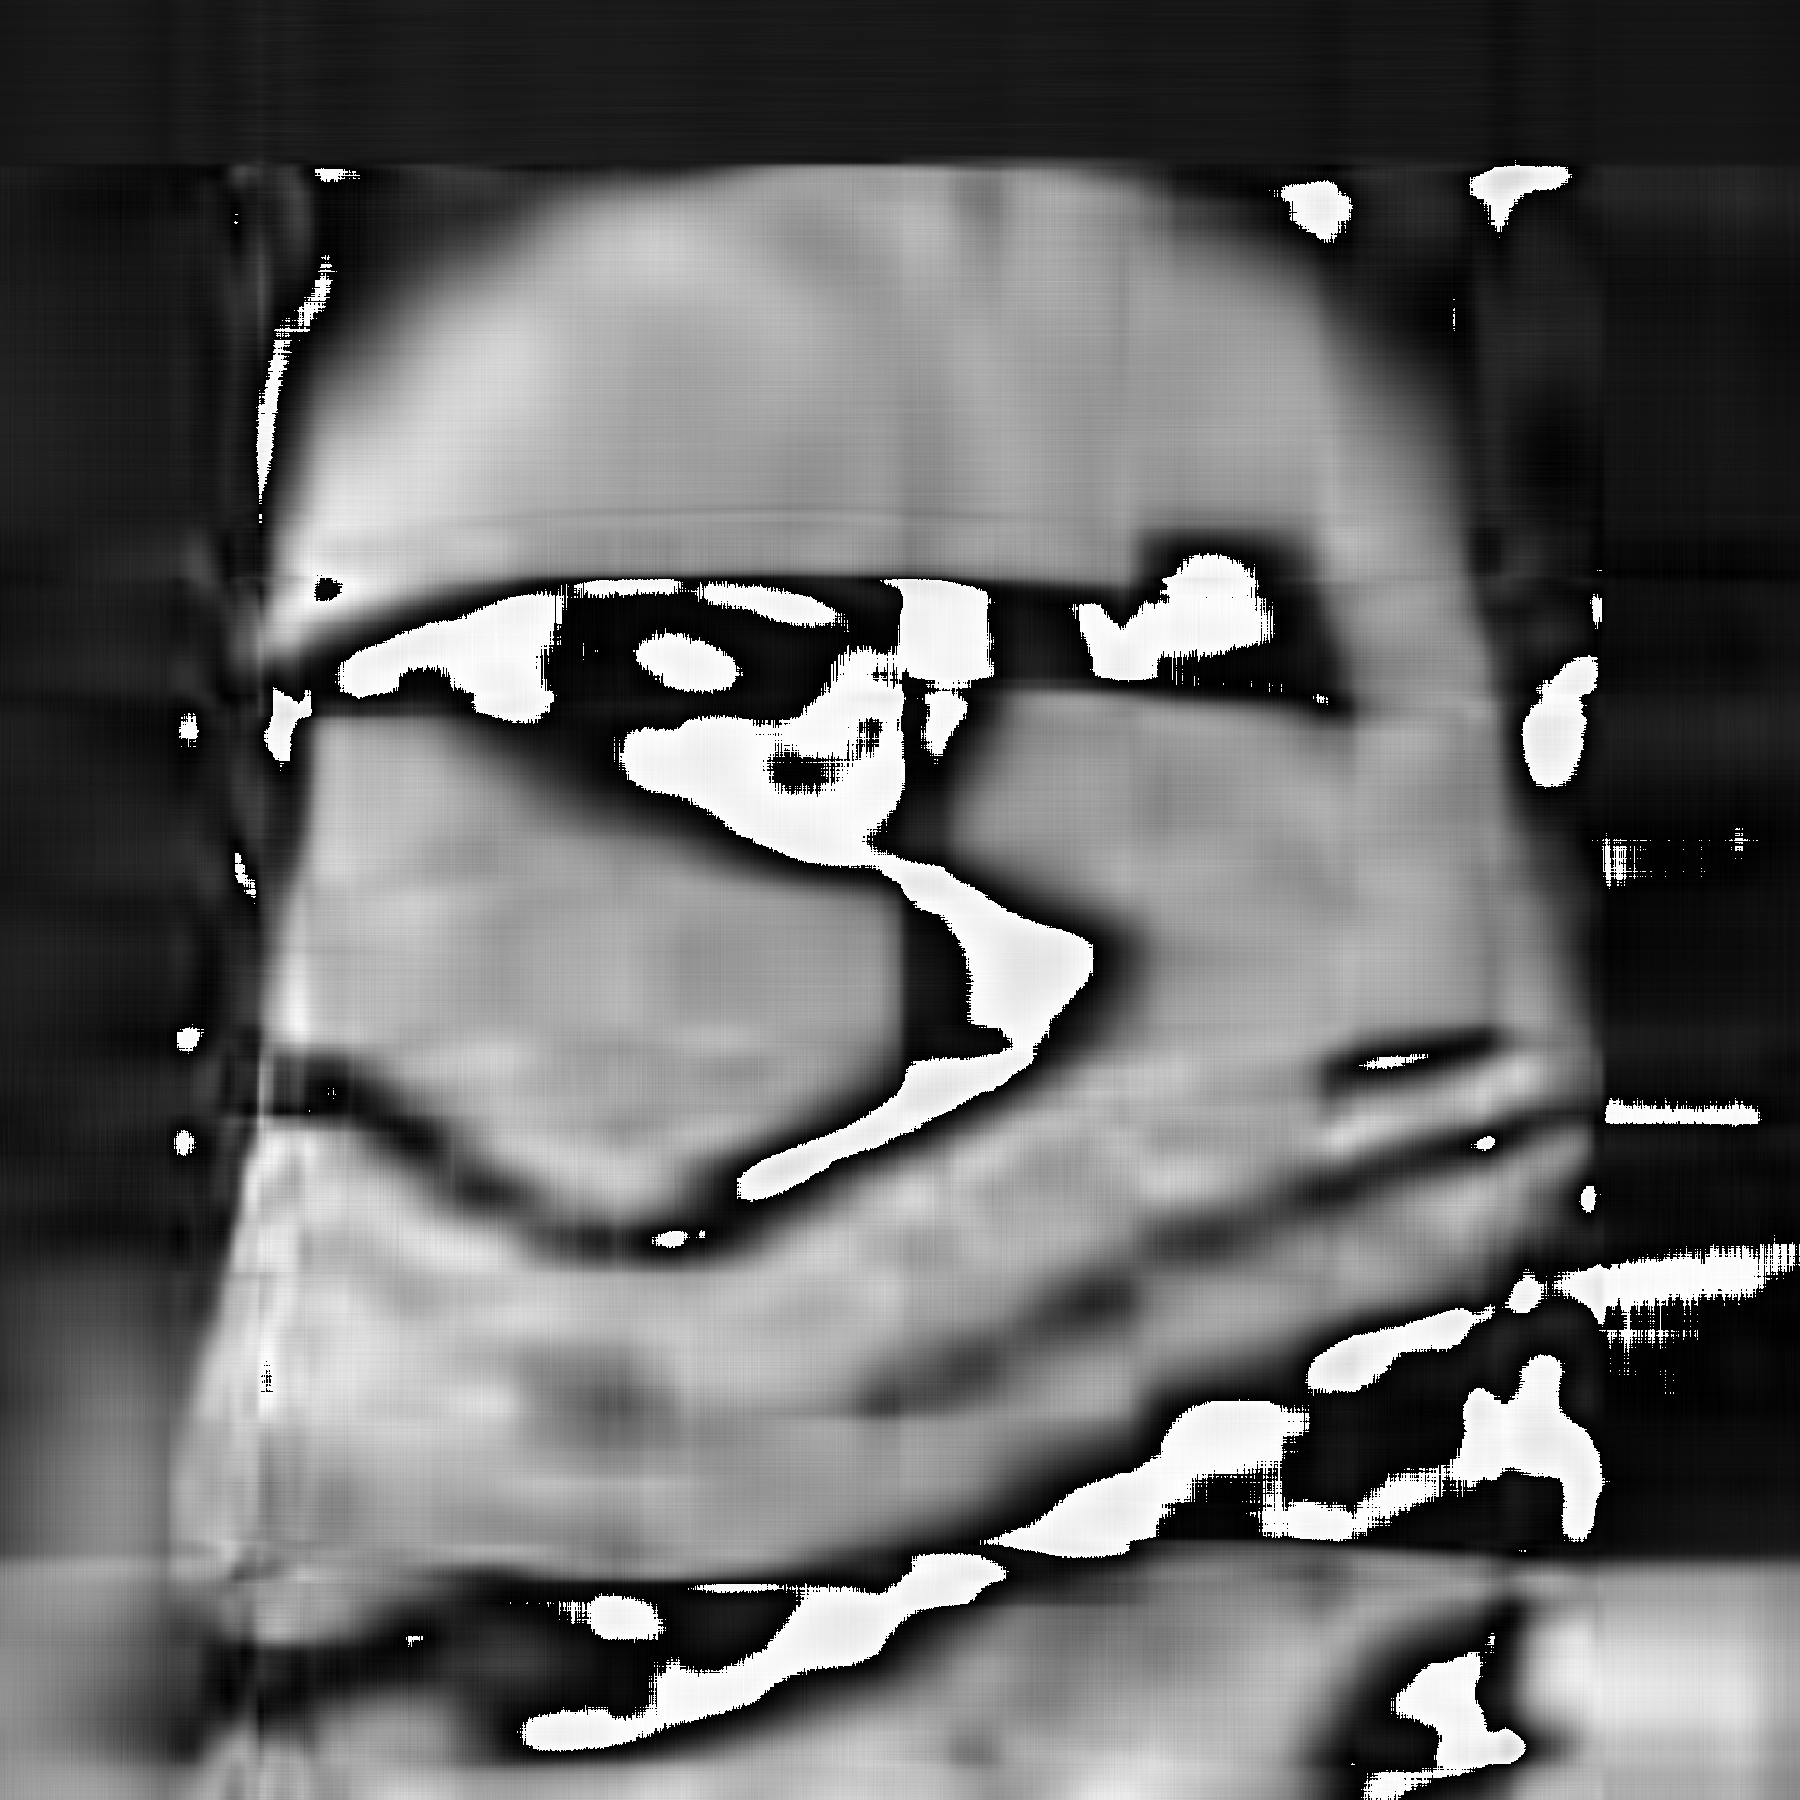
\includegraphics[width=0.3\textwidth]{approx12.png}\\
\smallskip
\scriptsize{Rank-20 (72,000 bytes)} &
\scriptsize{Rank-30 (108,000 bytes)} &
\scriptsize{Rank-40 (144,000 bytes)} \\

\includegraphics[width=0.3\textwidth]{approx20.png} &

\includegraphics[width=0.3\textwidth]{approx30.png} &
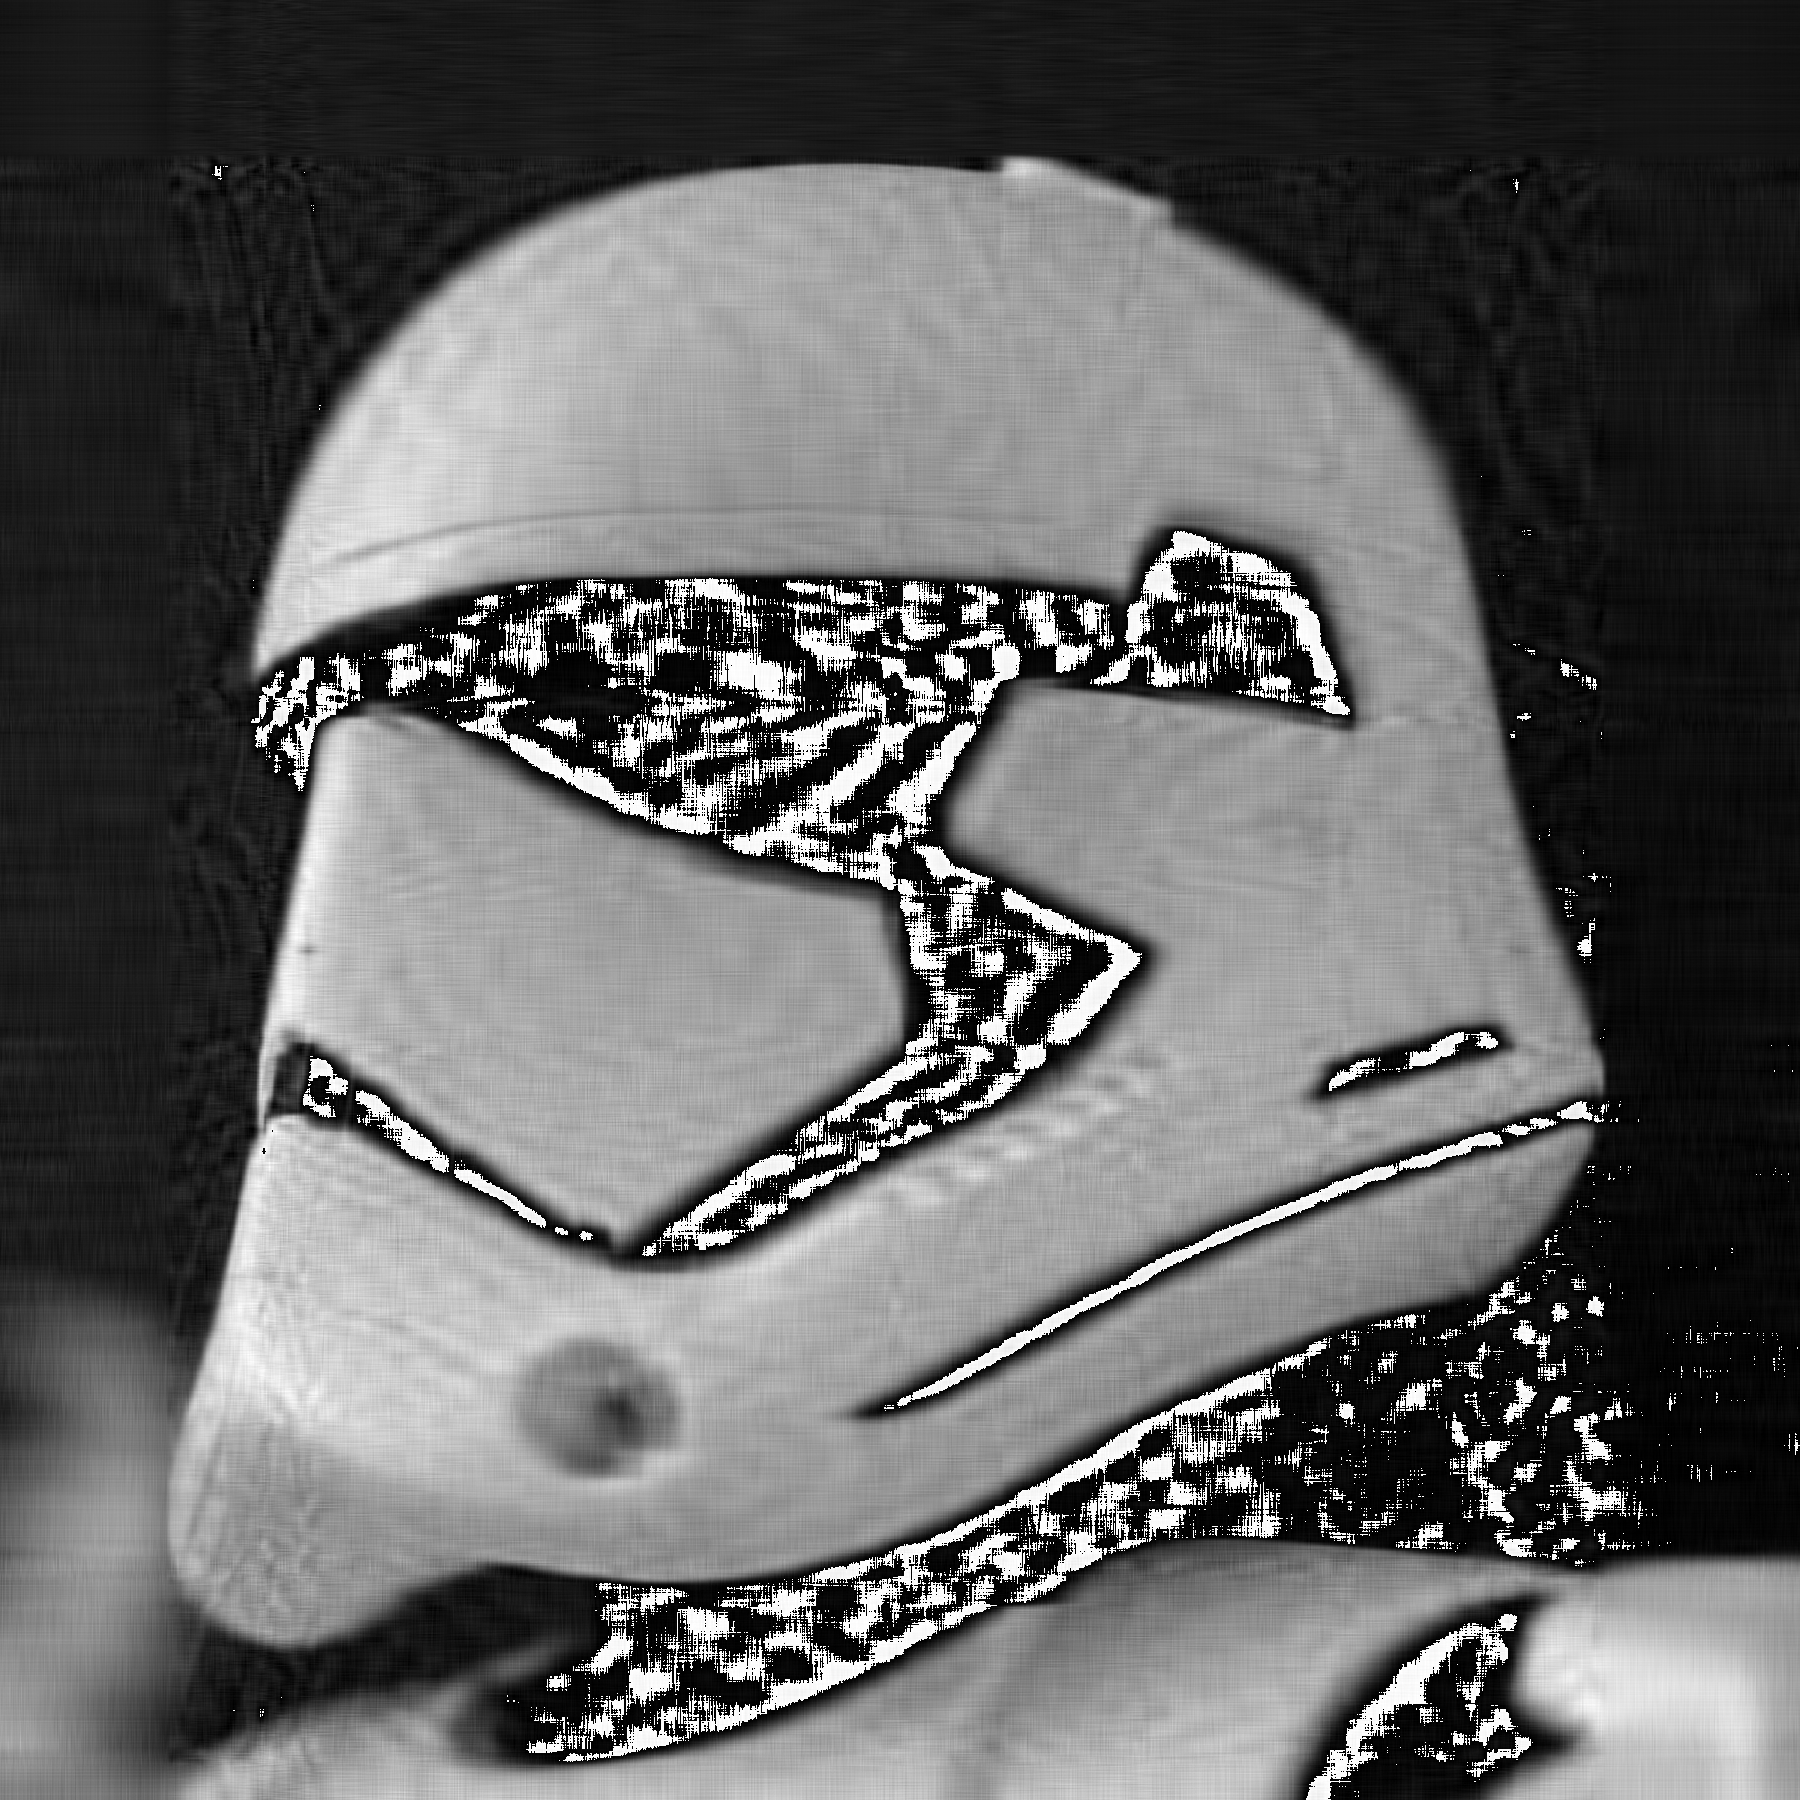
\includegraphics[width=0.3\textwidth]{approx40.png}\\
\scriptsize{Rank-100 (360,000 bytes)} &
\scriptsize{Rank-200 (720,000 bytes)} &
\scriptsize{Rank-400 (1,440,000 bytes)} \\
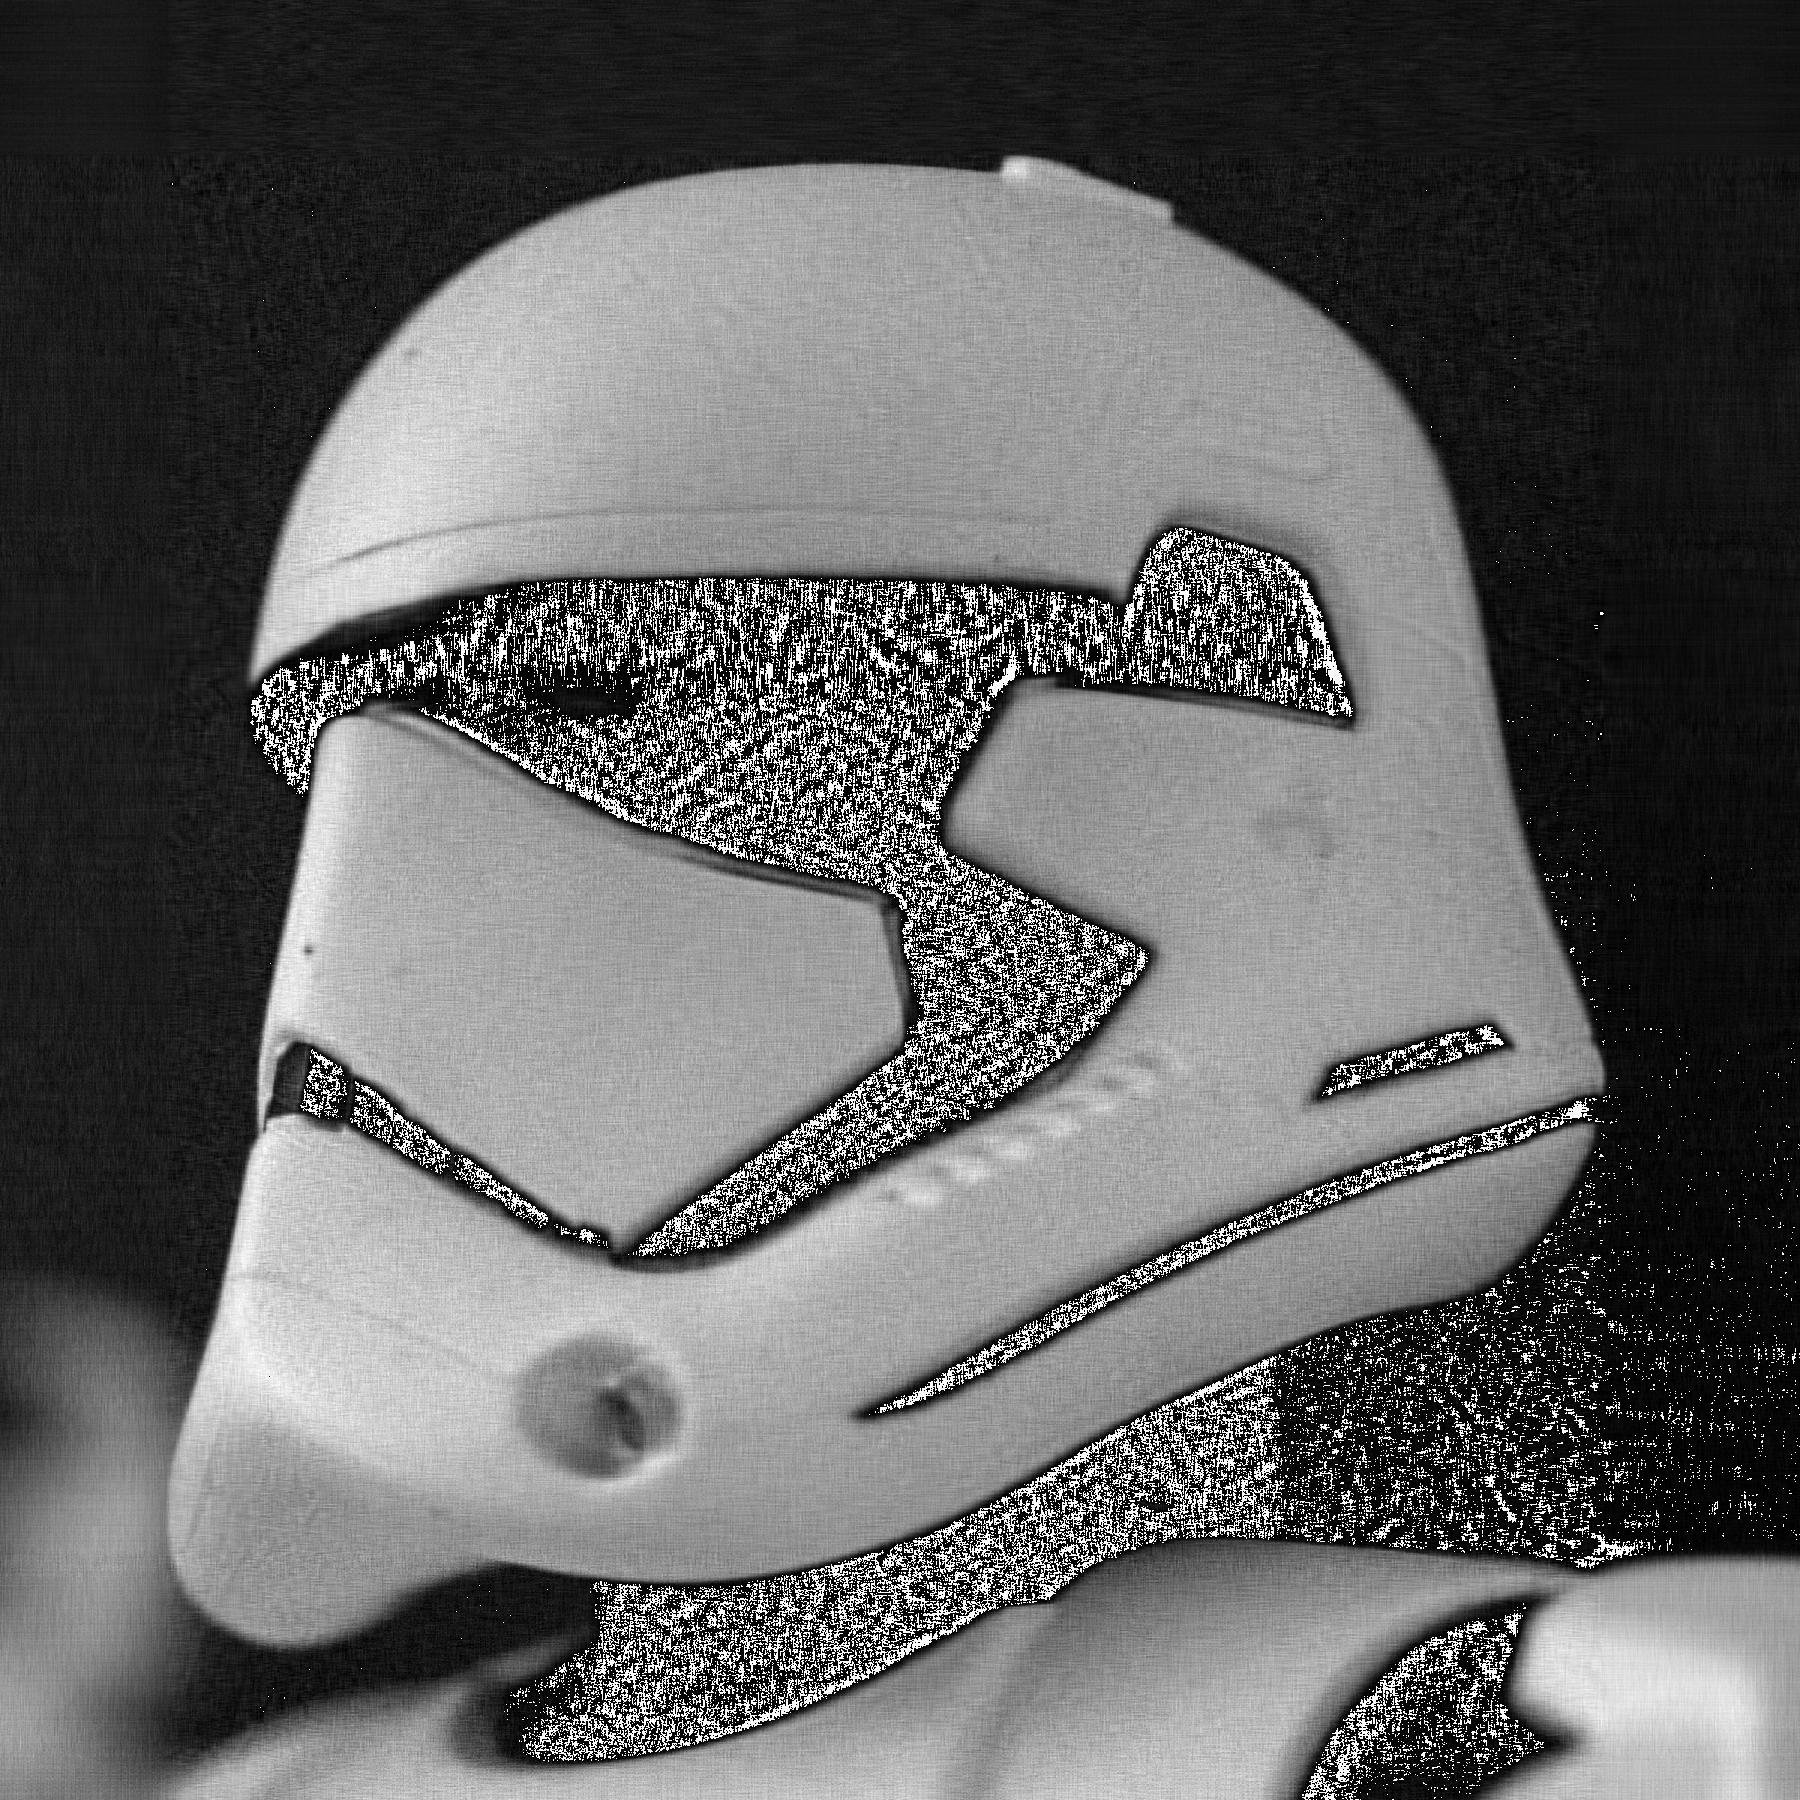
\includegraphics[width=0.3\textwidth]{approx100.png} &
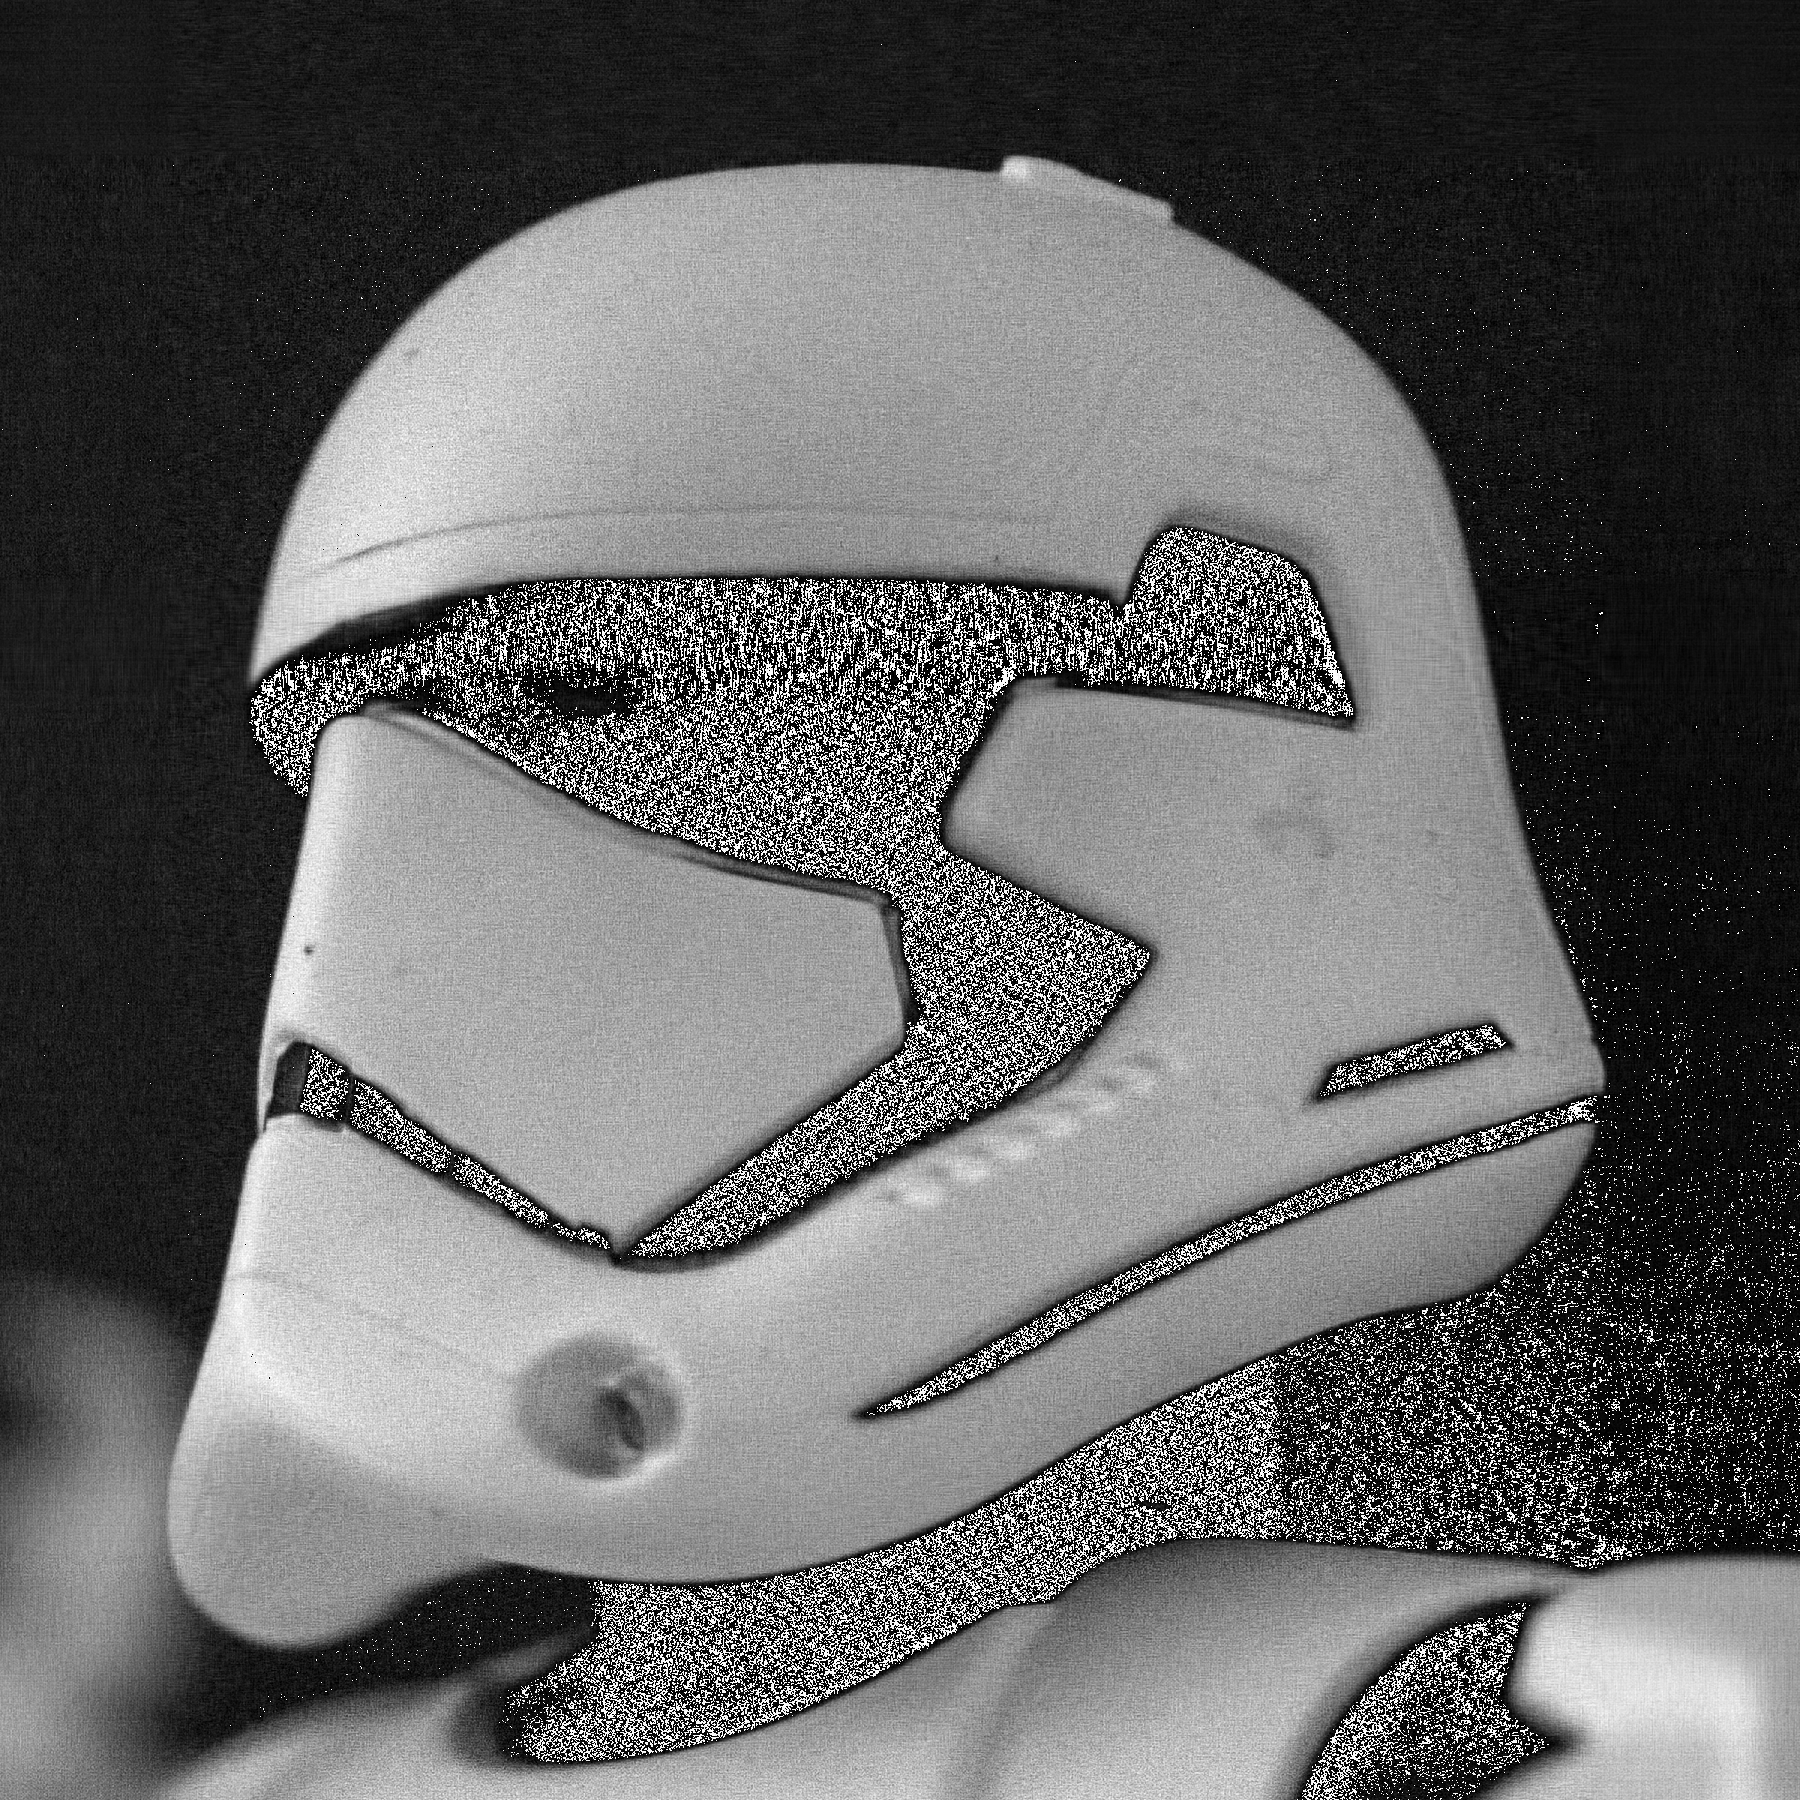
\includegraphics[width=0.3\textwidth]{approx200.png} &
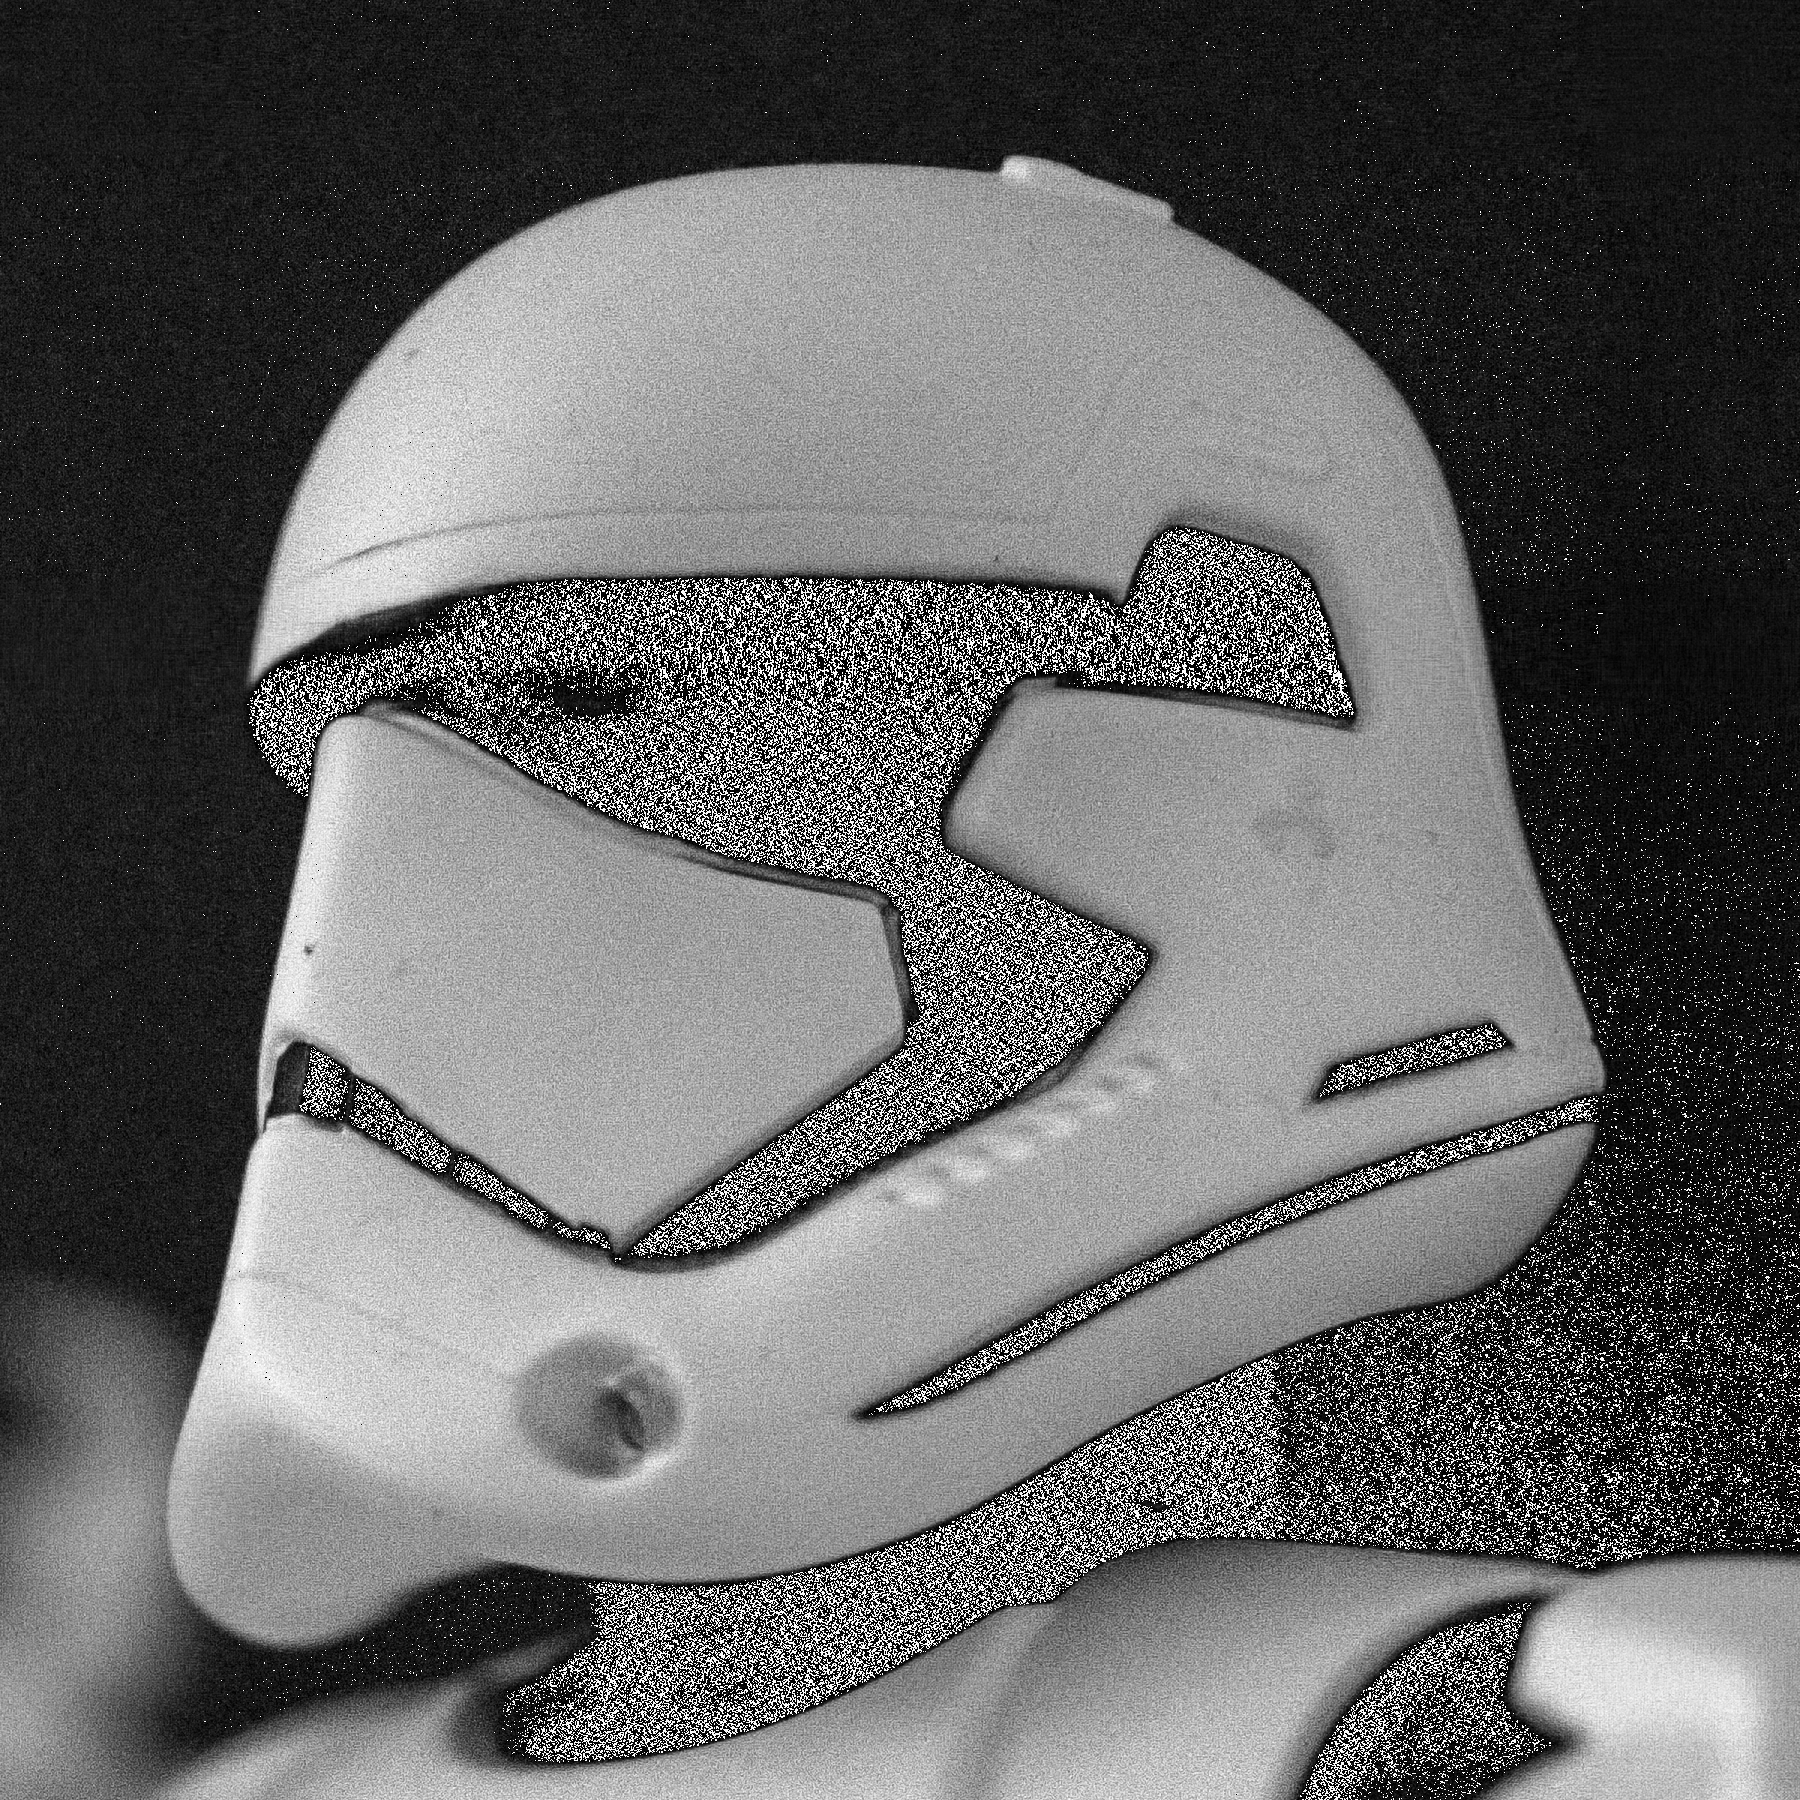
\includegraphics[width=0.3\textwidth]{approx400.png}\\
\end{tabular}
\caption{Low-rank approximations of an image matrix, using increasing numbers
of eigenvectors (and thus an increasing rank, with increasing
storage/transmission costs.)}
\label{fig:approximations}
\end{figure}

\pagebreak

It's interesting to watch how the image emerges as we add more eigenvectors.
With only the dominant eigenvector, all we can make out is a blurry,
right-angle-centric splash of black and white. Still, it's not bad for a rank-1
matrix, and after adding just a few more eigenvectors we can already see the
basic shape of the helmet come through.

Another observation is that we pretty quickly reach a point of diminishing
returns. Compare the rank-100 and rank-400 matrices in the bottom row of
Figure~\ref{fig:approximations}. Is it really worth quadrupling the size to get
the second one?

\begin{figure}[H]
\centering
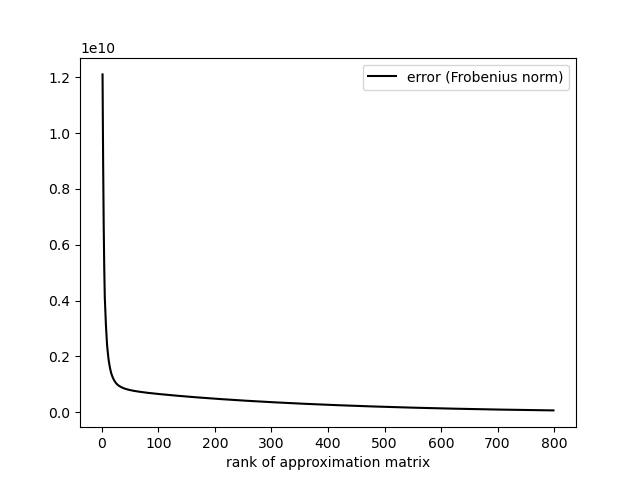
\includegraphics[width=0.7\textwidth]{frobenius.png}
\caption{The closeness to the original matrix as a function of the
approximation's rank.}
\label{fig:frobenius}
\end{figure}

Figure~\ref{fig:frobenius} quantifies this by plotting the rank of the matrix
against the Frobenius norm of the difference from the original. As you can see, 
less than fifty or so eigenvectors (out of the total of 1800) is enough to
eliminate nearly all the error.

\vfill
\pagebreak

\renewcommand{\thesubsection}{M\arabic{subsection}.}%... from subsections
\section{Markov chains}

\index{probability}

For our next eigenapplication, we'll need to review a few concepts from
Chapter 4 of \textit{A Cool Brisk Walk}: probability.

Recall that we can quantify the likelihood of some event happening by assigning
it a \textbf{probability} between 0 and 1, where 0 means the event is
impossible and 1 means it's a certainty. We use the notation ``Pr($E$)'' for
this, where $E$ is some event. Sometimes the probability is based on actual
counts of past occurrences, and sometimes it is estimated based on intuition
and common sense. For instance:

\begin{center}
Pr(home team wins in college basketball) = .6765 \\
\smallskip
Pr(worldwide pandemic next year) = .1
\end{center}

\index{conditional probability}

You may also recall the notion of \textbf{conditional probability}, in which
our estimate of an event's likelihood changes based on some other event being
known to have (or have not) occurred. We use the notation ``Pr($A|B$),''
pronounced as ``the probability of $A$ given $B$'' for this. Examples:

\begin{center}
Pr(speeding ticket) = .05 \\
\smallskip
Pr(speeding ticket\ $|$\ driving a red car) = .15 \\[12pt]
\medskip
Pr(Jets win tomorrow) = .7 \\
\smallskip
Pr(Jets win tomorrow\ $|$\ starting QB hurt in practice) = .4 \\
\end{center}

In one of these examples the conditional probability is higher than the
original, and in the other case it's lower, but either way it's always between
0 and 1.

\subsection{Systems and states}

\index{system}
\index{state}
\index{Monopoly}

Now recall from Chapter~\ref{ch:apps} that we often want to predict how the
\textbf{state} of some \textbf{system} will unfold over its lifetime. A
system's ``state'' is just a way of talking about the (temporary) condition it
is in at any one point in time. In this section, we're going to focus on just a
single aspect of a system's state, which has a single value at a point in time,
not a bunch of stuff like in the Monopoly example. Perhaps our system is the
U.S. economy, and in any given quarter its ``state'' is whether or not it's in
a recession. Or maybe we're interested in the system of local weather
conditions, for which each day's state is either sunny, cloudy, or rainy.

\index{independence}

Let's expand on this last example because we all have so much experience with
weather. One way we could get a handle on what tomorrow may bring is to count
how many days in the past have been sunny, cloudy, and rainy in our region, and
then assume \textbf{independence} between days. Remember that if two events are
independent, that means that the outcome of one of them has no impact on the
other. A Little League player's \textsl{jersey color} and \textsl{position} are
independent of each other: if you tell me Henry's uniform is blue, that doesn't
give me any information about whether he's an infielder or a pitcher.

So assuming independence, we could count up the past 100 days in
Fredericksburg, and conclude:

\vspace{-.15in}
\begin{align*}
\textrm{Pr(sunny)} &= .5 \\
\textrm{Pr(cloudy)} &= .4 \\
\textrm{Pr(rainy)} &= .1 \\
\end{align*}
\vspace{-.25in}

With this simple model, if someone asked us ``how likely is it to rain
tomorrow?''~we'd reply ``about a 10\% chance,'' no matter what the weather was
today, yesterday, or any other day. We figure that it doesn't matter what
happened on those other days, because we're assuming every day is independent
of the others.

Now this simplistic response is unsatisfying on several levels. For one, it
doesn't take into account the season we're in, mushing all months together into
a mediocre gray. But more to the point, it doesn't even take into account the
recent past. As we've all observed, weather patterns tend to form and transform
on a slower time scale than individual days. If it's hot today, it's pretty
likely to remain hot for at least a little while -- we're probably not going to
get a string of hot, cold, hot, cold, hot, and cold days consecutively.

\index{Markov chain}
\index{Markov property}
\index{Markov, Andrey}
\index{first-order}
\index{Ren, Kylo}
\index{Kylo Ren}
\index{Supreme Leader Snoke}

Remember that when the current state of some system is influenced only by its
\textit{previous} state, it has the so-called ``Markov property.'' In this
case, we can build a powerful structure called a \textbf{first-order Markov
chain} to analyze it. Markov chains are named for the brilliant Russian
mathematician Andrey Markov, one of the most underrated minds in history, in my
opinion. The phrase ``first order'' here has nothing to do with Kylo Ren or
Supreme Leader Snoke; it means that the system's current state depends only on
its immediately preceding state, and is conditionally independent of all states
longer ago than that.\footnote{If we said that a system's current state
depended on its immediately \textit{two} preceding states, we'd built a
second-order Markov chain, and so forth.} In weather terms, this means knowing
that it rained on Tuesday tells you something important about whether it will
also rain on Wednesday, but nothing (directly) about Thursday or beyond.

\subsection{Stochastic matrices}

A Markov chain can be modeled as (surprise!)~a matrix, which encodes all its
\textit{conditional probabilities}. Each one says: ``if the previous state is
$X$, here's the probability that the current state will be $Y$.''

For example, maybe it's true that heat waves tend to last longer than a day. If
it was sunny yesterday, it's likely to remain sunny today. In symbols, we might
say:

\vspace{-.15in}
\begin{align*}
\textrm{Pr(sunny}_k\ |\ \textrm{sunny}_{k-1}) &= .7 \\
\end{align*}
\vspace{-.25in}

The $k$ subscript is just to number the days. This formula says: ``the chances
of it being sunny on any particular day, given that it was sunny the day
before, are 70\%.''

\smallskip

Perhaps it's also true in our region that rainstorms tend not to last longer
than one day. (Once a storm finally breaks, the atmosphere has ``gotten the
rain out of its system'' and drier days will likely follow.) So we might
estimate these quantities:

\vspace{-.15in}
\begin{align*}
\textrm{Pr(rainy}_k\ |\ \textrm{rainy}_{k-1}) &= .05 \\
\textrm{Pr(cloudy}_k\ |\ \textrm{rainy}_{k-1}) &= .55 \\
\textrm{Pr(sunny}_k\ |\ \textrm{rainy}_{k-1}) &= .4 \\
\end{align*}
\vspace{-.25in}

We've saying that two rainy days in a row are very unlikely: if it rained
yesterday, it's most likely to be cloudy (and dry) today, not wet again.

\index{mutually exclusive}
\index{collectively exhaustive}

Note carefully that the above three numbers \textit{add up to exactly 1}, as
they must. The weather on day $k$ must either be rainy, cloudy, or sunny in our
simple weather model. Since these three possibilities are mutually exclusive
and collectively exhaustive, their probabilities must total 1.

\smallskip

If you nodded to the previous paragraph, make sure you also understand that the
\textit{following} three numbers do \textit{not} have to add up to 1 (and
normally won't):

\vspace{-.15in}
\begin{align*}
\textrm{Pr(cloudy}_k\ |\ \textrm{rainy}_{k-1}) &= .55 \\
\textrm{Pr(cloudy}_k\ |\ \textrm{cloudy}_{k-1}) &= .6 \\
\textrm{Pr(cloudy}_k\ |\ \textrm{sunny}_{k-1}) &= .2 \\
\end{align*}
\vspace{-.25in}

% WARNING: "top of the page"

Students sometimes get confused here. The three expressions look an awful lot
like the ones at the top of the page, yet the bottom three don't represent
mutually exclusive and collectively exhaustive options at all. The first of the
bottom three says ``what's the probability it'll be cloudy today if it was
rainy yesterday?'' The second asks a question about a completely different
circumstance: ``what about if it was \textit{cloudy} yesterday? Now how likely
are clouds today?'' These two numbers (.55 and .6) are unrelated to one
another, and not bound by any probability axioms.

\bigskip

And now, the matrix. There are nine different conditional probabilities for
this system, and we'll arrange them in a matrix called $W$ (for ``weather'') as
follows:

\vspace{-.2in}
\[
\begin{blockarray}{ccccccccc}
& & & & \leftarrow & {\overrightarrow{\textrm{day}_{k-1}}} & \rightarrow \\[11pt]
& & & & {\footnotesize\textrm{sunny}} & {\footnotesize\textrm{cloudy}} &
{\footnotesize\textrm{rainy}} \\
\begin{block}{cccc[ccccc]}
& & \uparrow & {\footnotesize\textrm{sunny}} & .7 & .3 & .4 \\
{\large W =} \quad\quad\quad & & {\textrm{day}_k} \ \ & {\footnotesize\textrm{cloudy}} & .2 & .6 & .55 \\
& & \downarrow & {\footnotesize\textrm{rainy}} & .1 & .1 & .05 \\
\end{block}
\end{blockarray}
\]

% WARNING: "last couple of pages"
The columns correspond to yesterday's weather, and the rows correspond to
today's weather. So if it was cloudy yesterday, the probability of sun today is
.3 (top-middle entry). If it was sunny yesterday, the probability of rain today
is .1 (bottom-left corner). Take a moment to look at this matrix and verify
your understanding of what each entry means. Also verify that the example
numbers on the previous couple of pages have all been entered in the right
places.

\index{stochastic matrix}
\index{probability matrix}
\index{substitution matrix}
\index{transition matrix}

A matrix of the form above goes by many names: some call them \textbf{Markov
matrices}, others \textbf{probability matrices}, still others
\textbf{transition matrices}, and yet others \textbf{substitution matrices}.
Me? I like the term \textbf{stochastic matrices} (since it sounds cool) so
that's what we'll go with here. (``Stochastic,'' by the way, is a word that
basically means ``random'' or ``indeterminate.'' Any time you're dealing with
probability, you have a stochastic system.)

\index{Leslie matrix}

Just like our Leslie matrices from p.~\pageref{sec:leslie} did, stochastic
matrices have certain constraints they must adhere to in order to join the
club. For a matrix to be a stochastic matrix:

\begin{compactenum}
\item all its entries must between 0 and 1, and
\item the sum of each of its columns must be exactly 1.
\end{compactenum}

(Notice I wrote ``the sum of each \textit{column},'' not row, for the same
reason I took pains to explain a few paragraphs ago. The rows don't normally
sum to 1, and there's no reason they should.)

Before going further, take a moment and verify that the $W$ matrix above is
indeed a stochastic matrix.

Then, complete this puzzle. Given the stochastic matrix $W$, which of the
following weeks of weather is most likely to actually occur? And which is least
likely? (``S''=sunny, ``C''=cloudy, ``R''=rainy)

\label{markovPuzzle}

\begin{adjustwidth}{38pt}{30pt}
\begin{multicols}{2}
\begin{compactenum}[a.]
\item S-R-S-R-S-R-S
\item S-R-R-R-S-S-S
\item S-C-S-C-S-C-S
\item S-S-S-S-C-C-C
\end{compactenum}
\end{multicols}
\end{adjustwidth}

(Answers on p.~\pageref{markovPuzzleSol}.)

\subsection{Simulating the Markov chain}

\index{linear operator}

The $W$ matrix is square, and thus a linear operator. It can be multiplied by
$3\times 1$ column vectors to produce other $3\times 1$ column vectors. Its
domain is vectors that represent yesterday's weather, and its codomain is
vectors that represent today's weather.

Suppose yesterday -- which we'll call ``day 1'' since it's the first day we'll
consider -- was a sunny day. We now want to predict what the weather will be
today. If we create a column vector for yesterday that has 1 for ``sunny'' and
0 for the other weather options, all we need to do is multiply it by $W$, and
whammo:

\vspace{-.15in}
\begin{align*}
W \cdot \overrightarrow{\textrm{day}_1} = \overrightarrow{\textrm{day}_2}.
\end{align*}
\vspace{-.15in}

By the actual numbers, we get:
\[
\begin{blockarray}{cccccc}
& {\footnotesize\textrm{sunny}} & {\footnotesize\textrm{cloudy}} &
{\footnotesize\textrm{rainy}} \\
\begin{block}{c[ccccc]}
{\footnotesize\textrm{sunny}} & .7 & .3 & .4 \\
{\footnotesize\textrm{cloudy}} & .2 & .6 & .55 \\
{\footnotesize\textrm{rainy}} & .1 & .1 & .05 \\
\end{block}
\end{blockarray} \cdot
\begin{bmatrix}
1 \\ 0 \\ 0 \\
\end{bmatrix} =
\begin{bmatrix}
.7 \\ .2 \\ .1
\end{bmatrix}.
\]

We set $\overrightarrow{\textrm{day}_1}$ to $[\ 1\ \ 0\ \ 0\ ]^\intercal$
because we \textit{knew} yesterday's weather. When we set out to make our
forecast, we knew that there was a 100\% chance it was sunny yesterday, and 0\%
chance it was either cloudy or rainy.

The resulting $\overrightarrow{\textrm{day}_2}$ vector, of course, does not
turn out to have only 0's and 1's. That's because the forecast is uncertain.
What the $\overrightarrow{\textrm{day}_2}$ vector means is that there will be a
10\% chance of rain today, a 20\% chance of overcast skies, and a 70\% chance
of clear blue.

Just like with Leslie matrices, we can run this forward any number of times we
want to predict into the distant future. Let's find out what the weather is
likely to be on day 4 (the day after tomorrow):

\vspace{-.15in}
\begin{align*}
W \cdot \overrightarrow{\textrm{day}_1} &= \overrightarrow{\textrm{day}_2} \\
W \cdot \overrightarrow{\textrm{day}_2} &= \overrightarrow{\textrm{day}_3} \\
W \cdot \overrightarrow{\textrm{day}_3} &= \overrightarrow{\textrm{day}_4} \\
\textrm{so} \\
W^3 \cdot \overrightarrow{\textrm{day}_1} &= \overrightarrow{\textrm{day}_4}.
\end{align*}
\vspace{-.15in}

\index{associative (operation)}

That last step takes advantage of the associative property of matrix
multiplication. This yields:

\[
\begin{blockarray}{cccccc}
& {\footnotesize\textrm{sunny}} & {\footnotesize\textrm{cloudy}} &
{\footnotesize\textrm{rainy}} \\
\begin{block}{c[ccccc]}
{\footnotesize\textrm{sunny}} & .5455 & .4815 & .49575 \\
{\footnotesize\textrm{cloudy}} & .35925 & .42325 & .409125 \\
{\footnotesize\textrm{rainy}} & .09525 & .09525 & .095125 \\
\end{block}
\end{blockarray} \cdot
\begin{bmatrix}
1 \\ 0 \\ 0 \\
\end{bmatrix} =
\begin{bmatrix}
.5455 \\ .35925 \\ .09525
\end{bmatrix}.
\]

Apparently, then, on the day after tomorrow we have only about a 55\% chance of
sunny weather. That is, if it had been sunny yesterday. What if it had been
cloudy yesterday?


\[
\begin{blockarray}{cccccc}
& {\footnotesize\textrm{sunny}} & {\footnotesize\textrm{cloudy}} &
{\footnotesize\textrm{rainy}} \\
\begin{block}{c[ccccc]}
{\footnotesize\textrm{sunny}} & .5455 & .4815 & .49575 \\
{\footnotesize\textrm{cloudy}} & .35925 & .42325 & .409125 \\
{\footnotesize\textrm{rainy}} & .09525 & .09525 & .095125 \\
\end{block}
\end{blockarray} \cdot
\begin{bmatrix}
0 \\ 1 \\ 0 \\
\end{bmatrix} =
\begin{bmatrix}
.4815 \\ .42325 \\ .09525
\end{bmatrix}.
\]

Given cloudy weather yesterday, our forecast for the day after tomorrow would
look even bleaker: just a 48\% chance of sun.

\subsection{...and eigenvectors}

Now what does all of this have to do with eigenvectors? So far, all this neat
Markov chain material could have been in Chapter~\ref{ch:apps} before we'd
learned about eigenstuff.

Well, if you haven't guessed it, the key insight is related to the diagrams in
Section~\ref{magneticPull} (``Magnetic pull,'' p.~\pageref{magneticPull}).
Remember that when we took any old vector, and repeatedly multiplied a square
matrix by it, the answers we got out were sucked closer and closer to the
matrix's dominant eigenvector, as if by magic.

Realize that's exactly what we're doing here with this forecasting-the-future
stuff. We started with a vector of 0's and 1's representing the actual weather
on a particular day, and we multiplied it by $W$ once for each day we wanted to
project our forecast into the future. This means that the further into the
future we go, the forecast is going to inevitably be drawn to $W$'s dominant
eigenvector.

Python tells us that the dominant eigenvector for our matrix $W$ is:

\vspace{-.15in}
\begin{align*}
\overrightarrow{x_1} = \begin{bmatrix} .5159 \\ .3889 \\ .0952 \end{bmatrix},
\ \ \textrm{with} \ \lambda_1 = 1.
\end{align*}
\vspace{-.15in}

Believe it or not, this vector gives us \textbf{the long-run distribution of
the states in the weather system.} Up until now, we've been extrapolating from
yesterday's weather out two or three days. But suppose I said, ``okay, let's
just say a year goes by. What's the probability on any given future day that
we'll have sunny, cloudy, or rainy weather?'' The answer is given in that
magical eigenvector $\overrightarrow{x_1}$. On days far in the future, there
will be precisely a 51.59\% chance of sun, a 38.89\% chance of clouds, and a
9.52\% chance of showers.

\index{initial condition}

This is the long-run behavior of the Markov chain, dissected and exposed.

It's interesting to think about the fact that it only depends on the $W$ matrix
itself, not on the starting vector we used for
$\overrightarrow{\textrm{day}_1}$ (such a starting point is often called an
\textbf{initial condition}). If you think about it, it makes a lot of sense. If
we're projecting the long-running behavior of a system, many many days in the
future, should it really matter whether \textit{today} happened to be sunny,
cloudy, or rainy? Surely predictions way out in the future shouldn't rely any
longer on any one observation in the distant past. Its influence has long since
faded to nothing. And that's exactly what we find. If you're trying to predict
the weather a few days from now, it's worth it to consider what yesterday's
weather was and extrapolate out from that. But if you're interested in planning
your wedding weekend for next summer, that's just too far out for yesterday's
weather to matter. The eigenvector will keep your forecast honest.

\vfill
\pagebreak

\renewcommand{\thesubsection}{W\arabic{subsection}.}%... from subsections
\section{Web search}

\index{search engine}
\index{Web search}

We end this chapter, book, and series with a look at one of the most
influential algorithms in world history. It's called
``PageRank,''\footnote{PageRank was invented by \index{Page, Larry}
\index{Brin, Sergey} \index{Google} Larry Page and Sergey Brin, the founders of
Google. I always wondered if Sergey was jealous that the algorithm wasn't
called ``BrinRank.'' Wdyt?} and it's what made Google Google. Like the other
applications in this chapter, it's based on eigenvectors. First, though, let's
take a look at the state of the art before PageRank.

\subsection{Web search: pre-Google}
\label{sec:webSearchPreGoogle}

\index{Yahoo\!}

It's interesting to study the history of Web search engines, which we don't
have time to do here. But one thing you should know is the approach that Google
used to dominate the market. Before Google, search engines (like Yahoo!,
Excite, and Alta Vista) focused only on returning results that matched your
search terms well.

\index{Jezebel}
\index{Filbert}
\index{matchmaker@\texttt{matchmaker.com}}

Remember all the way back to the beginning of this book
(p.~\pageref{matchmakerExample} and following), where we discussed a matchmaker
dating application for Jezebel, Filbert, and friends. Each person took a survey
of interests, and was thereafter represented by a single vector of numbers,
which represented how well they liked hiking, candlelight dinners, and so
forth. To determine the compatibility between two people, we simply computed
the dot product of their two vectors. This worked because in order for a dot
product to be large, the two vectors have to have large entries in the same
slots of the vector.

\index{Mr.~Right}
\index{normalizing (a vector)}

One wrinkle with this approach, which we analyzed on
pp.\pageref{matchmakerGameTheSystemStart}-\pageref{matchmakerGameTheSystemEnd},
was that it was possible for someone to game the system by simply answering 10
to all the questions. The way to counteract this insidious strategy was to
\textit{normalize} everyone's vector before computation. This way, each person
effectively only has a certain total ``amount'' of ``interests'' which they
have to spread among their answers.

\index{word count}
\index{cnn.com@\texttt{cnn.com}}

Interestingly, this is almost exactly the approach used by Web search engines
to gauge the similarity between two pages, or the similarity of a page to a
search query. Each Web page is represented as a vector of numbers. In place of
survey responses as the vector elements, substitute \textbf{word counts}.
That's right: for every word that appears on any Web page anywhere, a page's
vector has an entry for \textit{the number of times that word appears on that
page.} So the vector corresponding to (say) \texttt{cnn.com}'s home page today
might be:

\vspace{-.15in}
\begin{center}
\begin{tabular}{cccccccc}
$\overrightarrow{\textbf{cnn.com}}$ \ = [ & 105 & 0 & 1 & 3 & $\cdots$ & 0 & ] \\
& \scriptsize{a} & \scriptsize{aardvark} & \scriptsize{abolish} &
\scriptsize{abstention} & $\cdots$ & \scriptsize{zoology} & \medskip \\
\end{tabular}
\end{center}
\vspace{-.15in}

\index{aardvark}
\index{zoology}
\index{bag of words}

This would indicate that the text on \texttt{cnn.com} has 105 instances of the
word ``a,'' no ``aardvarks,'' one ``abolish,'' three ``abstentions,'' and so
forth: one entry for every possible word.\footnote{This might seem like a
prohibitively huge number to you at first, but it's really not. The English
language, for instance, only has about half a million words in it, and that's
if you count absolutely \textit{everything}, even obscure words that haven't
been used since the 15th century. Throw in all the proper nouns, trademarks,
slang terms, misspellings, abbreviations, plus the words in every
\textit{other} language on earth and you're still just in the low millions.
Contrast that with the number of \textit{pages} there are on the Web, which is
in the billions.} Notice we're deliberately throwing away the information about
the \textit{order} words appear on the page. All we care about is how many
times each word appears. This is called the ``\textbf{bag of words}'' model,
since it's like taking scissors to the page, cutting up all the individual
words, and dropping them in a bag. It turns out to work very well in practice.

After forming this vector for a page, we then play the same trick we did on
Jezebel \& Co., which is to normalize it:

\vspace{-.15in}
\begin{center}
\begin{tabular}{ccccccc}
$\overrightarrow{\textbf{cnn.com}}$ \ = [ & \footnotesize{.0249} &
\footnotesize{0} & \footnotesize{.000237} & \footnotesize{.000711} & $\cdots$ &
\footnotesize{0} \quad ] \\
& \scriptsize{a} & \scriptsize{aardvark} & \scriptsize{abolish} &
\scriptsize{abstention} & $\cdots$ & \scriptsize{zoology} \quad \medskip \\
\end{tabular}
\end{center}
\vspace{-.15in}

This tells us that about 2.5\% of all the words on \texttt{cnn.com} today are
the word \texttt{a}, .0237\% of them are the word \texttt{abolish}, and so on.
We're thus summing up the content of the page by saying: ``this
\texttt{cnn.com} page is 2.5\% `about' the word \texttt{a}, .0237\% `about' the
word \texttt{abolish}, \textit{etc.}''

\index{Potter, Harry}
\index{Harry Potter}

Now, if I wanted to find ``pages with similar content to \texttt{cnn.com},''
I'd calculate the dot product of every page's (normalized) vector with CNN's
vector, and take the highest results. Or, if a Yahoo!~user entered
``\texttt{harry potter the sorcerers stone}'' in the search box, I'd first make
a vector on the fly with a 1 for each of the five words of the query and 0
everywhere else, then normalize it, and finally take its dot product with every
page's vector. Effectively, this means I'd be looking for the pages for which
the percentage of words that are \texttt{harry}, \texttt{potter}, \texttt{the},
\texttt{sorcerers}, or \texttt{stone} is the highest.

\medskip

I'm glossing over several other pragmatic steps that search engines take to
improve the accuracy of their results. Among them are:

\vspace{-.1in}
\begin{itemize}

\item Getting rid of punctuation, capitalization, and other stuff that doesn't
pertain to the root meanings of a word.

\index{stemming}

\item Collapsing all different forms of the same root word to a single entry.
In English, this is called \textbf{stemming}, because we're finding the word's
stem and using it instead of the raw word. The idea here is that the words
\texttt{jump}, \texttt{jumps}, \texttt{jumped}, and \texttt{jumping} all
reflect the same basic meaning. If we're trying to capture the topics of a Web
page, we really don't care which of the specific variants of the word appear,
only its root meaning.

\index{stop list}

\item Dropping super-common words altogether. Words like ``\texttt{a},''
``\texttt{the},'' and ``\texttt{of}'' don't actually hold any meaningful
content, because every page has zillions of them regardless of what it's about.
Search engines use a \textbf{stop list} of common words to discard.

\index{TF/IDF}

\item Scaling the importance of each word by how common it is. This is a
gentler version of the previous item, but it's very important. The idea is that
the more common a word is, the less about the page it tells you by being
present on it.

Consider these two words, for example: \texttt{dollar}, and \texttt{Jedi}. If I
chose a random Web page and told you only that it contained the word
\texttt{dollar}, how much would you know about its content? Some, but not much.
But if I told you that it contained the word \texttt{Jedi}, how much would you
know? A lot more. This is because \texttt{dollar} is a more common word, and
therefore appears in many more different contexts than the word \texttt{Jedi}
does. A popular algorithm for this is called \textbf{TF/IDF}, which stands for
``term frequency / inverse document frequency.'' The amount that a vector's
entry contributes to the dot product is the frequency of that word in the page
(\textit{i.e.}, how many times \texttt{abstention} or a variant of it appears
in that page) divided by that word's frequency appearing in documents
(\textit{i.e.}, what percentage of all Web pages that \texttt{abstention}
appears on). Words like \texttt{dollar} will appear in a much higher percentage
of Web pages, and thence be ``discounted'' more steeply when it comes to
computing similarity to queries.

\end{itemize}

\subsection{Web search: Google}

Now let's take a step back. All of the details in the previous section were
devoted to one strategy: find Web pages whose \textit{content} matches the
user's search terms well. The entire purpose of a search engine (everyone
thought before 1998) was to identify relevant documents for the user, and
``relevant'' meant ``the words on the page are a good match for what the user
typed.''

\index{popularity}

When Google came on the scene in 1998, they of course did all that
content-matching stuff too. But they added a critical second component to the
criteria for ranking search results. In a way, I've always thought their new
ingredient was kind of depressing, but in the end it turned out to be what
the world really wanted. The key second ingredient was to factor in the
\textbf{popularity} of a page, in addition to its content.

\index{Rowling, J.K.}
\index{Potter, Harry}
\index{Harry Potter}

Simply put, Google realized that in addition to wanting pages that match their
search terms, users also want pages that are well-known and in some sense
authoritative. They want to be channeled towards the pages that everyone else
already knows about and likes. I find this depressing because it seems to
encourage a herd mentality, and to discourage the discovery of new information.
But the fact of the matter is that when I type ``\texttt{harry potter the
sorcerers stone}'' in a search box, most of the time I don't want to read the
Web page of some random crazy Harry Potter fan from Greenland. Instead, I want
the IMDB page from the movie, or J.K.Rowling's site that discusses her ideas,
or the Wikipedia page describing the book's release and its reception. In a
word, I want the popular websites.

That was Page's and Brin's first innovation: to factor popularity into search
results, so that even if a big well-known website didn't match the search terms
as well as a lesser-known website did, it would get funneled up to the top of
the results list anyway.

\subsection{The PageRank algorithm}

So their first innovation was to take into account a page's popularity at all.
Their second one was in how to \textit{determine} the popularity of a page. A
good illustration here is to think of the drama on a middle school playground.
Everyone knows that a school has popular kids, and not-so-popular kids. (I
was one of the latter.) A first cut at measuring this could be expressed as
follows:

\vspace{-.1in}
\begin{center}
First try: \textit{``You're popular if a lot of kids like you.''}
\end{center}

\index{hyperlink}

Now if we substitute Web pages for kids, this formula gives us some hope of
quantifying the popularity of a Web page. All we have to do is figure out what
one page ``liking'' another page really means. And I'll bet you can figure it
out if you just think about it for a moment. The way page A can ``like'' page B
-- the way it can vouch for page B's awesomeness, or authoritativeness, or
whatever -- is simply to \textbf{link} to it. Most every Web page has embedded
hyperlinks in it, so that when you click on a word or a button you're
transported to another page. So we can measure a page's popularity by how many
other pages have a link to it:

\vspace{-.1in}
\begin{center}
First try: \textit{``A page is popular if lots of other pages link to it.''}
\end{center}

That simple idea is almost PageRank. Almost. But the killer feature of Google's
algorithm was to add one little word to the middle school popularity contest.
Here it is:

\vspace{-.1in}
\begin{center}
PageRank: \textit{``You're popular if a lot of \textbf{popular} kids like you.''}
\end{center}

Or, expressed in terms of the Web:

\vspace{-.1in}
\begin{quote}
PageRank: \textit{``A page is popular if lots of other \textbf{popular} pages link to it.''}
\end{quote}

\index{dweeb}

Yeah, that does pretty much match my experience, I have to admit. If the dweebs
and the losers like you, that doesn't say very much. But if kids who are
themselves well-liked and admired by others express admiration for
\textit{you}, that's a gold-plated imprimatur.

\subsection{Calculating the PageRank vector}

Now as true as the above definition of popularity rings, you may rightly object
that it seems circular. We want to measure how popular Sam is. And we know that
popular kids are liked by lots of popular kids...but how could we determine how
popular Sam's admirers are themselves without getting in an infinite loop?

Eigenvectors will turn out to solve this problem for us. Like. Magic.

\index{graph}
\index{adjacency matrix}

To get there, remember your graphs from \textit{A Cool Brisk Walk} Chapter 5,
or from p.~\pageref{sec:graphs} of this book. The World Wide Web is nothing
other than a gigantic directed graph, where each vertex is a Web page and each
edge is a hyperlink. Here's a tiny tiny example of one:

\begin{center}
\includegraphics[width=0.5\textwidth]{web.pdf}
\end{center}

In this minuscule ``Web'' of just four pages, page A has a link to page B, page
B has links to each of the other three, page C has links to B and D, and page D
has only a link to page C.

Remember also from p.~\pageref{firstAdjacencyMatrix} that we can represent a
graph by its adjacency matrix $A$. This square matrix has one row/column for
each vertex of the graph, and a 1 in the positions with an edge from one vertex
to another. In this case, the matrix is:

\[
A_{\textrm{mini-Web}} = 
\begin{blockarray}{ccccc}
& {\footnotesize\textrm{A}} & {\footnotesize\textrm{B}} & {\footnotesize\textrm{C}} & {\footnotesize\textrm{D}} \\
\begin{block}{c[cccc]}
{\footnotesize\textrm{A}} & 0 & 1 & 0 & 0 \\
{\footnotesize\textrm{B}} & 1 & 0 & 1 & 1 \\
{\footnotesize\textrm{C}} & 0 & 1 & 0 & 1 \\
{\footnotesize\textrm{D}} & 0 & 0 & 1 & 0 \\
\end{block}
\end{blockarray}.
\]

(Run your eyeballs over that matrix, and compare it with the graph, before
continuing.)

\medskip

\index{PageRank vector}

We're going to compute what's known as the \textbf{PageRank vector} for this
graph. It will have one numeric entry for each Web page, which will represent
the popularity of that page.

Here's how to do it.

First, we'll do some light bookkeeping on the $A_{\textrm{mini-Web}}$ matrix,
by (1) taking its transpose and then (2) normalizing the columns. We'll call
this revised matrix $M$:

\begingroup
\renewcommand*{\arraystretch}{1.2}
\[
M_{\textrm{mini-Web}} = 
\begin{blockarray}{ccccc}
& {\footnotesize\textrm{A}} & {\footnotesize\textrm{B}} & {\footnotesize\textrm{C}} & {\footnotesize\textrm{D}} \\
\begin{block}{c[cccc]}
{\footnotesize\textrm{A}} & 0 & \frac{1}{3} & 0 & 0 \\
{\footnotesize\textrm{B}} & 1 & 0 & \frac{1}{2} & 0 \\
{\footnotesize\textrm{C}} & 0 & \frac{1}{3} & 0 & 1 \\
{\footnotesize\textrm{D}} & 0 & \frac{1}{3} & \frac{1}{2} & 0 \\
\end{block}
\end{blockarray}.
\]
\endgroup

\index{transpose}
\index{Manhattan norm}

I used the Manhattan norm here to make the numbers easier on the eyes, but any
other norm would be okay too. Note that the sum of each column is 1.

Now here's how to interpret $M$. Each column corresponds to one page's
``praise'' for the other pages in the Web. And that page has a total of
\textit{one} ``praise point'' to spend on this praise. In the first column, we
see that page A has put all its eggs in one basket: it's screaming loudly that
page B, and only page B, is important. That's because in the graph, A has only
one outgoing link (which is to B). In the second column, by contrast, page B
has spread its praise equally across pages A, C, and D -- since it has links to
all three of those. Page C divvies up its praise between B and D, while D
shouts loudly for C and only C.

The rationale behind normalizing the columns should now be apparent to you.
It's the matchmaker leveling effect in action again. A page can have as many
outgoing links as it wants, but the more it has, the less potent each one will
be in determining popularity.

\medskip

\index{random surfer}
\index{surfer}

To get your head around PageRank, try to visualize a \textbf{random surfer}
mindlessly clicking links in his browser as he surfs the Web. Imagine that
this surfer started with some arbitrary page, and then he chose one of its
links at random and clicked on it. Then he chose one of \textit{that} page's
links at random and clicked on it, and continued that process indefinitely.
(You should try this at home -- it's usually rather amusing where you end up
after a minute or two, no matter what page you started on.)

The key question to ask is this: after the random surfer does his thing for a
few hours, what's the probability that he lands on page A? What about B? C? D?

Let's work it out mathematically. We'll create a vector
$\overrightarrow{\textbf{p}}$ that contains, for each page, the probability
that the random surfer will be on that page. The process starts with a
completely random page, remember, so we have a $\frac{1}{4}$ probability of
starting on each:

\vspace{-.2in}
\begin{align*}
\overrightarrow{p}_1 =
\begin{bmatrix}
.25 \\
.25 \\
.25 \\
.25 \\
\end{bmatrix}.
\end{align*}
\vspace{-.2in}

The ``1'' subscript says that these are the probabilities for the
\textit{first} page the random surfer browses.

Okay, what's the probability that the \textit{second} page he browses is each
of the four?

\index{Law of Total Probability}

If you remember your Law of Total Probability from \textit{A Cool Brisk Walk},
you'll know that the probability of visiting page A second is:

\vspace{-.15in}
\begin{align*}
\textrm{Pr(page A second)}\ =\ &\textrm{Pr(page A second}\ |\ \textrm{page A
first)}\ + \\
                             &\textrm{Pr(page A second}\ |\ \textrm{page B
first)}\ + \\
                             &\textrm{Pr(page A second}\ |\ \textrm{page C
first)}\ + \\
                             &\textrm{Pr(page A second}\ |\ \textrm{page D first)}.
\end{align*}
\vspace{-.15in}

In other words, there are four different ways that page A could be my second
destination; namely, my first two pages could have been AA, BA, CA, or DA.

Do you see how to get the probability of this -- and also the probability of
landing on any of the other pages second -- from the $M$ matrix? It's a snap.
All you do is matrix-vector multiplication! $\overrightarrow{\textbf{p}_2}$ is
simply $M \cdot \overrightarrow{\textbf{p}_1}$.

\vspace{-.15in}
\begin{center}
$\overrightarrow{p}_2 = M \cdot \overrightarrow{p}_1 = 
\begin{bmatrix}
0 & \frac{1}{3} & 0 & 0 \\
1 & 0 & \frac{1}{2} & 0 \\
0 & \frac{1}{3} & 0 & 1 \\
0 & \frac{1}{3} & \frac{1}{2} & 0 \\
\end{bmatrix} \cdot
\begin{bmatrix}
.25 \\
.25 \\
.25 \\
.25 \\
\end{bmatrix} =$ \\
\medskip
$.25 \cdot
\begin{bmatrix}
0 \\
1 \\
0 \\
0 \\
\end{bmatrix} +
.25 \cdot
\begin{bmatrix}
.333 \\
0 \\
.333 \\
.333 \\
\end{bmatrix} +
.25 \cdot
\begin{bmatrix}
0 \\
.5 \\
0 \\
.5 \\
\end{bmatrix} +
.25 \cdot
\begin{bmatrix}
0 \\
0 \\
1 \\
0 \\
\end{bmatrix} = 
\begin{bmatrix}
.083 \\
.375 \\
.333 \\
.208 \\
\end{bmatrix}.
$
\end{center}
\vspace{-.15in}

I'm using the ``second way'' of thinking about matrix-vector multiplication
here (from p.~\pageref{twoInterpretations}) -- a linear combination of $M$'s
columns. Since there's a $\frac{1}{4}$ chance of being on page A first, and
page A always goes to page B, that means there's a .25 probability of starting
the random surf with the sequence AB, and a 0 probability of starting with AA,
AC, or AD. So when constructing our totals, we add .25 times $[\ 0\ \ 1\ \ 0\ \
0\ ]^\intercal$.

There's also a $\frac{1}{4}$ probability of starting on page B. But if that
happens, then there's a $\frac{1}{3}$ chance (each) of going to A, C, or D
next. Put that together, and you see that there's a $\frac{1}{12}$ probability
of starting with any of the BA, BC, or BD sequences, and a 0 probability of
starting with BB. \textit{Etc.} Repeat that process, and you get the
$\overrightarrow{\textbf{p}}_2$ result shown above: a 37.5\% chance of landing
on page B second, nearly that high a chance (33.3\%) of landing on page C
second, and smaller likelihoods (8.3\% and 20.8\%, respectively) of landing on
page A or D second.

What about how likely each page is to be \textit{third} in the sequence? Just
multiply by $M$ again to get $\overrightarrow{\textbf{p}_3}$.

What about fourth? Just multiply by $M$ again to get
$\overrightarrow{\textbf{p}_4}$. 

What about fifth? Just multiply by $M$ again to get
$\overrightarrow{\textbf{p}_5}$. 

\textit{(\dots and so on \dots)}

And now for the finishing touch. What about the \textit{long-term} likelihood
of visiting each of the pages? In other words, after the random surfer has been
doing his thing for a while, what do the probabilities settle down to?

What we're really asking for is $\overrightarrow{\textbf{p}_\infty}$. This
would seem to require infinite multiplications to compute the value of
$M^\infty \cdot \overrightarrow{\textbf{p}_1}$. But remember the magic of
eigenvectors: if you keep multiplying $M$ by \textit{any} vector, it will be
drawn to the dominant eigenvector like a moth to the flame. So we don't have to
actually multiply infinitely many times, or even once; instead, we just take
$M$'s dominant eigenvector!

And that, my friends, is the PageRank vector. For the graph above, the dominant
eigenvector turns out to be:

\vspace{-.15in}
\begin{align*}
\overrightarrow{\textbf{pagerank}}_\textrm{mini-Web} =
\begin{bmatrix}
.159 \\
.286 \\
.305 \\
.249 \\
\end{bmatrix},
\end{align*}
\vspace{-.15in}

which announces with finality that C is officially the most popular page of the
bunch, with a PageRank score of .305, and that the others are B, D, and A, in
that order.

The PageRank algorithm vanquishes the circularity problem. We can safely define
popular pages as ``pages which lots of other popular pages link to'' yet not
get stuck in an infinite loop. All we need to do is calculate the dominant
eigenvector of the modified adjacency matrix, and we magically obtain the
popularity of every page in our Web.

Combining this popularity information with the relevancy information used by
older search engines (p.~\pageref{sec:webSearchPreGoogle}) is how Google
changed the world. It's why you can type any old thing into a search engine
these days and in the blink of an eye get exactly the pages you were looking
for. I search the Web many times every day, and I almost never need to go to
even the \textit{second} page of search results. The pages I want are
invariably at the top of the list. Who knew that steering me towards popular
pages would be exactly what I really wanted?

\vfill
\pagebreak

\subsection*{Answers to Markov chain puzzle from
p.~\pageref{markovPuzzle}}

Just by thinking about how we designed the probabilities, you can probably
eyeball that sequence d is the most likely and sequence b the least likely. In
sequence d, we have four sunny days in a row, followed by three cloudy days,
and it is in fact true that both sunny days and cloudy days like to follow each
other. In sequence b, though, we have four rainy days in a row which just
isn't going to happen very often, since our probability of two consecutive
rainy days is a mere .05.

Here's the precise numerical answers:

\begin{compactenum}[a.]
\small
\item
Pr(rainy$_2\ |\ $sunny$_1$) $\cdot$
Pr(sunny$_3\ |\ $rainy$_2$) $\cdot$
Pr(rainy$_4\ |\ $sunny$_3$) $\cdot$
Pr(sunny$_5\ |\ $rainy$_4$) $\cdot$
Pr(rainy$_6\ |\ $sunny$_5$) $\cdot$
Pr(sunny$_7\ |\ $rainy$_6$) $\\=
.1 \cdot .4 \cdot .1 \cdot .4 \cdot .1 \cdot .4 = $\ \textbf{.000064} \\
\item
Pr(rainy$_2\ |\ $sunny$_1$) $\cdot$
Pr(rainy$_3\ |\ $rainy$_2$) $\cdot$
Pr(rainy$_4\ |\ $rainy$_3$) $\cdot$\\
Pr(sunny$_5\ |\ $rainy$_4$) $\cdot$
Pr(sunny$_6\ |\ $sunny$_5$) $\cdot$
Pr(sunny$_7\ |\ $sunny$_6$) $\\=
.1 \cdot .05 \cdot .05 \cdot .4 \cdot .7 \cdot .7 = $\ \textbf{.000049} \\
\item
Pr(cloudy$_2\ |\ $sunny$_1$) $\cdot$
Pr(sunny$_3\ |\ $cloudy$_2$) $\cdot$
Pr(cloudy$_4\ |\ $sunny$_3$) $\cdot$
Pr(sunny$_5\ |\ $cloudy$_4$) $\cdot$
Pr(cloudy$_6\ |\ $sunny$_5$) $\cdot$
Pr(sunny$_7\ |\ $cloudy$_6$) $\\=
.2 \cdot .3 \cdot .2 \cdot .3 \cdot .2 \cdot .3 = $\ \textbf{.000064} \\
\item
Pr(sunny$_2\ |\ $sunny$_1$) $\cdot$
Pr(sunny$_3\ |\ $sunny$_2$) $\cdot$
Pr(sunny$_4\ |\ $sunny$_3$) $\cdot$
Pr(cloudy$_5\ |\ $sunny$_4$) $\cdot$
Pr(cloudy$_6\ |\ $cloudy$_5$) $\cdot$
Pr(cloudy$_7\ |\ $cloudy$_6$) $\\=
.7 \cdot .7 \cdot .7 \cdot .2 \cdot .6 \cdot .6 = $\ \textbf{.024696} \\

\end{compactenum}

Take special note that even though weeks a and b have the same number of rainy
and sunny days, the order makes all the difference. Since rainy days don't like
to follow each other, sequence a is more likely to occur than sequence b. By
contrast, weeks c and d have the same number of sunny and cloudy days, but
since those types of weather \textit{do} like to follow each other, sequence d
is far more likely.

\label{markovPuzzleSol}


\end{alttitles}
